\documentclass[11pt]{article}

\usepackage[margin=1in]{geometry}
\usepackage{fontspec}
\setmainfont{Times New Roman}
\usepackage{graphicx}
\usepackage{booktabs}
\usepackage{array}
\usepackage{xcolor}
\usepackage{hyperref}
\usepackage{caption}
\usepackage{float}
\usepackage{amsmath}
\usepackage{enumitem}
\usepackage{titlesec}
\usepackage{fancyhdr}
\usepackage{longtable}
\usepackage{multirow}
\usepackage{parskip}
\usepackage{microtype}
\usepackage{polyglossia}
\setmainlanguage{vietnamese}

\emergencystretch=3em
\sloppy

\hypersetup{colorlinks=true, linkcolor=black, citecolor=black, urlcolor=blue, pdftitle={Bai tap 04 - So sanh cac cach cai dat CNN va MLP}}

\pagestyle{fancy}
\fancyhf{}
\fancyfoot[C]{\thepage}
\renewcommand{\headrulewidth}{0pt}
\renewcommand{\footrulewidth}{0pt}

\titleformat{\section}{\normalfont\Large\bfseries}{\thesection}{1em}{}
\titleformat{\subsection}{\normalfont\large\bfseries}{\thesubsection}{1em}{}
\titleformat{\subsubsection}{\normalfont\normalsize\bfseries}{\thesubsubsection}{1em}{}

\newcommand{\model}[1]{\textbf{#1}}
\newcommand{\code}[1]{\texttt{#1}}
\newcommand{\impl}[1]{\textbf{#1}}

\begin{document}

% ---------------------------------------------------------------------
% Trang bìa
% ---------------------------------------------------------------------
\begin{titlepage}
\centering
\vspace*{2cm}
{\Large PHÁT TRIỂN HỆ THỐNG THÔNG MINH}\\[0.3cm]
{\Large BÀI TẬP 04}\\[0.5cm]
{\huge \bfseries So sánh các cách cài đặt CNN và MLP: Viết tay (Scratch) vs. Keras vs. PyTorch}\\[2cm]

\begin{tabular}{ll}
Họ tên sinh viên: & Nguyễn Văn Trường \\[0.5cm]
Mã số sinh viên: & B23DCCE095 \\[0.5cm]
Lớp: & E23CNPM02 \\[0.5cm]
Môn học: & Phát triển hệ thống thông minh \\[0.5cm]
Giảng viên: & PGS. TS. Đinh Quế Trân \\[0.5cm]
Học kỳ: & I.2026 \\
\end{tabular}

\vfill
{\large Ba ứng dụng, một MLP và hai CNN, mỗi ứng dụng được xây dựng và huấn luyện
ba lần riêng biệt: viết tay bằng NumPy, bằng TensorFlow/Keras, và bằng PyTorch,
nhằm so sánh mức độ trừu tượng của cách cài đặt chứ không phải để so sánh các
mô hình với nhau.}
\end{titlepage}

\tableofcontents
\newpage

% ---------------------------------------------------------------------
\section{Tóm tắt tổng quan}
% ---------------------------------------------------------------------

Báo cáo này xây dựng ba hệ thống thông minh: sàng lọc nguy cơ tiểu đường
(dữ liệu dạng bảng, phân loại nhị phân), nhận diện trang phục Fashion-MNIST
(ảnh xám, phân loại 10 lớp), và nhận diện vật thể CIFAR-10 (ảnh màu RGB,
phân loại 10 lớp), mỗi ứng dụng dùng \textbf{một kiến trúc duy nhất} nhưng được
cài đặt ba lần riêng biệt: viết tay bằng NumPy không dùng bất kỳ framework
deep learning nào, bằng TensorFlow/Keras, và bằng PyTorch. Mục tiêu của bài
tập \textbf{không phải} là tìm ra mô hình tốt nhất trong chín mô hình đã huấn
luyện. Mục tiêu là kiểm chứng trực tiếp luận điểm trung tâm của Lecture 04:
cùng một bài toán học máy, được biểu diễn bằng cùng một kiến trúc, phải cho
ra kết quả gần giống nhau bất kể được xây dựng ở mức độ trừu tượng nào trong
ba mức đó, và cái thực sự khác nhau giữa ba cách cài đặt là mức độ hiển thị
của code, sự tiện lợi cho người phát triển, và tốc độ huấn luyện, chứ không
phải bản chất toán học bên dưới.

Bảng \ref{tab:exec-summary} tóm tắt ba ứng dụng và cách cài đặt nào thắng
theo độ chính xác trên tập kiểm tra (test accuracy) — chỉ số so sánh chính
của bài tập.

\begin{table}[H]
\centering
\caption{Tóm tắt tổng quan ba ứng dụng}
\label{tab:exec-summary}
\small
\begin{tabular}{@{}p{2.2cm}p{2.4cm}p{2.6cm}p{2.9cm}p{2.6cm}@{}}
\toprule
Ứng dụng & Loại dữ liệu & Bài toán & Kiến trúc & Cách cài đặt thắng \\
\midrule
Diabetes & dạng bảng & phân loại nhị phân & MLP ($50 \to 32 \to 16 \to 1$) & PyTorch (0.782) \\
Fashion-MNIST & ảnh, $28\times28\times1$ & phân loại 10 lớp & CNN (421.642 tham số) & Scratch (0.897) \\
CIFAR-10 & ảnh, $32\times32\times3$ & phân loại 10 lớp & CNN (545.098 tham số) & Keras (0.610) \\
\bottomrule
\end{tabular}
\end{table}

Có hai kết quả đáng được nêu bật trước khi đi vào từng phần chi tiết theo
ứng dụng bên dưới. Thứ nhất, mọi ứng dụng đều cho ra \textbf{đúng cùng một
số lượng tham số} ở cả ba cách cài đặt — một sự thật mà mỗi notebook không
chỉ giả định suông mà còn \textbf{chủ động kiểm tra}
(\code{assert keras\_param\_count == scratch\_param\_count}, và một phép
kiểm tra tương tự với PyTorch); đây là bước kiểm tra tính hợp lý (sanity
check) quan trọng nhất trong toàn bộ bài tập, vì nó xác nhận ba cách cài
đặt thực sự là \textbf{một kiến trúc duy nhất}, chứ không phải ba kiến trúc
không liên quan chỉ tình cờ trùng tên. Thứ hai, \textbf{không có cách cài
đặt nào áp đảo} ở mọi ứng dụng: PyTorch thắng ở Diabetes, scratch thắng ở
Fashion-MNIST, và Keras thắng ở CIFAR-10, với khoảng cách giữa người thắng
và các cách còn lại không bao giờ vượt quá vài điểm phần trăm accuracy
trong cả ba trường hợp. Thay vì làm suy yếu luận điểm của Lecture 04, thứ
hạng thay đổi liên tục này lại \textbf{ủng hộ} luận điểm đó, bởi vì nếu một
cách cài đặt duy nhất luôn thắng thì điều đó cho thấy có sự khác biệt thực
sự về năng lực mô hình hóa, trong khi thứ hạng xáo trộn từ ứng dụng này
sang ứng dụng khác chính xác là điều mà ba cách cài đặt có năng lực ngang
nhau của cùng một kiến trúc sẽ tạo ra, với kết quả được quyết định bởi
những chi tiết nhỏ ở cấp độ framework chứ không phải do cách cài đặt nào
đó có năng lực học vốn dĩ mạnh hơn. Thời gian huấn luyện là tín hiệu rõ
ràng hơn nhiều so với accuracy: Keras luôn hoàn thành nhanh nhất ở mọi ứng
dụng, và code NumPy viết tay từ đầu tụt lại rất xa so với hai cách còn lại
ngay khi có convolution thực sự tham gia — một cái giá cụ thể của việc
"hiển thị toàn bộ" mà MLP của bài Diabetes không hề lộ ra, vì mạng đó đủ
nhỏ để chi phí phụ trội (overhead) của bất kỳ cách cài đặt nào cũng không
đủ lớn để chiếm ưu thế.

% ---------------------------------------------------------------------
\section{Liên hệ với Lecture 04: Cùng kiến trúc, khác mức độ trừu tượng}
\label{sec:lecture}
% ---------------------------------------------------------------------

Phần này được viết một lần duy nhất, ở cấp độ khung lý thuyết chung, để ba
phần theo từng ứng dụng ở sau không phải suy diễn lại cùng một lập luận.
Mỗi phần theo ứng dụng bên dưới sẽ minh họa lại các ý tưởng được trình bày ở
đây bằng số liệu và code cụ thể của riêng nó, và sẽ tham chiếu đến phần này
thay vì lặp lại.

\subsection{Câu hỏi trung tâm}

Toàn bộ bài tập được đóng khung bởi một câu hỏi mà Lecture 04 mở đầu: trong
ba cách cài đặt cùng một CNN — NumPy viết tay từ đầu, TensorFlow/Keras, và
PyTorch — \textit{cái gì thực sự giữ nguyên, và cái gì thực sự thay đổi?}
Bài giảng trả lời trực tiếp: kiến trúc ở mức khái niệm hoàn toàn không thay
đổi giữa ba cách; chỉ có mức độ trừu tượng là thay đổi. Ở scratch, một
\code{Conv2d} là một hàm cụ thể thực hiện phép nhân ma trận kiểu
\code{im2col}, có thể đọc và theo dõi từng dòng. Ở Keras, cùng phép toán đó
rút gọn thành một dòng duy nhất, \code{Conv2D(...)}, với toàn bộ công việc
nhân-và-cộng-dồn (multiply-and-accumulate) được ẩn bên trong một thư viện
đã biên dịch sẵn. \code{nn.Conv2d(...)} của PyTorch nằm ở giữa hai thái
cực: việc định nghĩa layer gọn gàng như Keras, nhưng vòng lặp huấn luyện
gọi đến nó và lượt lan truyền ngược (backward pass) cập nhật nó vẫn phải
viết tường minh trong code của sinh viên, thay vì được gói gọn trong một
lệnh gọi \code{fit()} duy nhất.

\subsection{Khái niệm mới là thứ cần trùng khớp, chứ không phải tên gọi}

Lecture 04 nói rõ điều này: tên gọi khác nhau không có nghĩa là khái niệm
học máy khác nhau. Mọi cách cài đặt trong bài tập này đều diễn đạt cùng bảy
ý tưởng — convolution (chỉ ở các ứng dụng ảnh), activation, pooling (chỉ ở
các ứng dụng ảnh), flatten (chỉ ở các ứng dụng ảnh), một lớp dense/linear,
một hàm loss, và một bước cập nhật của optimizer — dưới một cái tên khác
nhau ở mỗi framework. Bảng \ref{tab:concept-api} nhắc lại chính bảng tương
ứng khái niệm-với-API của bài giảng, được rút gọn cho đúng phạm vi dự án
này sử dụng; phiên bản đầy đủ theo từng ứng dụng của bảng này xuất hiện ở
phần so sánh riêng của mỗi ứng dụng bên dưới (đúng yêu cầu của slide 28),
được điền bằng chính đoạn code mà mỗi cách cài đặt thực sự viết ra, chứ
không phải một chỗ trống mang tính minh họa chung chung.

\begin{table}[H]
\centering
\caption{Bảng tương ứng khái niệm–API dùng xuyên suốt dự án này}
\label{tab:concept-api}
\small
\begin{tabular}{@{}p{2.3cm}p{3.4cm}p{3.7cm}p{3.7cm}@{}}
\toprule
Khái niệm & Mục đích & Scratch & Keras / PyTorch \\
\midrule
Convolution & trích xuất đặc trưng cục bộ & \code{conv2d\_forward} (\code{im2col}) & \code{Conv2D} / \code{nn.Conv2d} \\
Activation & phi tuyến hóa & \code{relu()} & \code{"relu"} / \code{nn.ReLU()} \\
Pooling & giảm chiều không gian & \code{max\_pool2d\_forward} & \code{MaxPooling2D} / \code{nn.MaxPool2d} \\
Flatten & tensor $\to$ vector & reshape & \code{Flatten()} / \code{nn.Flatten()} \\
Dense/Linear & phân loại & \code{linear\_forward} (matmul) & \code{Dense} / \code{nn.Linear} \\
Loss & đo lường sai số & công thức viết tay & lớp loss của framework \\
Optimizer & cập nhật tham số & \code{W -= lr * dW} & \code{optimizer="sgd"} / \code{torch.optim.SGD} \\
\bottomrule
\end{tabular}
\end{table}

\subsection{Vị trí của mỗi cách cài đặt trên phổ mức độ hiển thị}

Scratch có mức độ hiển thị tối đa: mọi phép nhân, mọi gradient, và mọi lần
cập nhật tham số đều là code được viết tay và có thể đọc từng dòng, đổi lại
là khối lượng công việc cài đặt lớn nhất và, như kết quả bên dưới cho thấy
nhiều lần, thời gian huấn luyện chậm nhất một khi có convolution thực sự
tham gia. Keras có mức độ tiện lợi tối đa: định nghĩa mô hình chỉ là một
lệnh gọi \code{Sequential([...])}, và \code{model.fit(...)} sở hữu toàn bộ
vòng lặp huấn luyện, lượt lan truyền tiến, loss, lượt lan truyền ngược, và
cập nhật tham số — tất cả đều vô hình đối với code gọi nó. PyTorch cố tình
nằm ở giữa: định nghĩa layer gọn như Keras bên trong một \code{nn.Module},
nhưng vòng lặp huấn luyện (\code{zero\_grad} $\to$ forward $\to$ loss
$\to$ \code{backward()} $\to$ \code{step()}) vẫn tường minh trong code của
sinh viên, với đạo hàm tự động (\code{autograd}) chỉ đảm nhiệm việc tính
gradient, chứ không đảm nhiệm cả vòng lặp bao quanh nó.

\subsection{Quy tắc công bằng chi phối mọi so sánh bên dưới}

Lecture 04 nêu rõ ràng buộc để bất kỳ so sánh nào trong số này có ý nghĩa:
\textit{cùng dataset, cùng cách chia tập, cùng kiến trúc, siêu tham số
tương đương}. Mọi ứng dụng trong báo cáo này tuân theo quy tắc đó một cách
trực tiếp. Với mỗi ứng dụng, cách chia train/test, độ rộng và độ sâu của
các layer, kích thước batch, số epoch, và tốc độ học đều được cố định
\textbf{một lần}, trước khi bất kỳ cách cài đặt nào trong ba cách được xây
dựng, và được tái sử dụng không đổi ở cả ba. Điểm \textbf{duy nhất} mà dự
án này không giả định sự tương đồng tuyệt đối giữa các framework là
\textbf{khởi tạo trọng số}: cách cài đặt scratch dùng khởi tạo He tường
minh, có gieo seed (\code{np.random.randn(...) * sqrt(2/fan\_in)}, bias
bằng 0); Keras và PyTorch mỗi bên áp dụng bộ khởi tạo mặc định riêng, cả
hai cũng thuộc họ He/Kaiming phù hợp với ReLU, nhưng không đảm bảo cho ra
trọng số khởi đầu giống hệt bit-for-bit với công thức của scratch hay với
nhau. Sự khác biệt đó được xem là một nguồn phân kỳ \textbf{hợp lệ, đáng
được báo cáo} giữa các cách cài đặt trong các kết quả bên dưới, chứ không
phải điều cần che giấu hay giả định là không tồn tại.

\newpage
% ---------------------------------------------------------------------
\section{Diabetes: Phân loại nhị phân (MLP)}
\label{sec:diabetes}
% ---------------------------------------------------------------------

\subsection{Mô tả bài toán}

Ứng dụng này dự đoán xem một người tham gia khảo sát BRFSS (Behavioral Risk
Factor Surveillance System — Hệ thống giám sát yếu tố nguy cơ hành vi) có
bị tiểu đường hoặc tiền tiểu đường hay không, dựa trên các câu trả lời tự
khai về sức khỏe và nhân khẩu học. Đầu vào là một vector đặc trưng phẳng,
không có mối quan hệ không gian 2 chiều có ý nghĩa giữa các cột — BMI và
tình trạng hôn nhân không liên quan về mặt không gian với nhau theo cách mà
các pixel liền kề có — nên ứng dụng này dùng một mạng truyền thẳng thông
thường (MLP) thay vì CNN, đúng với lý do mà Lecture 04 đưa ra để giải thích
tại sao Diabetes không bao giờ dùng convolution: \textit{không có phép toán
convolution tự nhiên} cho loại dữ liệu dạng bảng này.

\subsection{Tập dữ liệu}

Tập dữ liệu gộp năm file dữ liệu đầy đủ theo từng năm từ bộ dữ liệu Kaggle
\begin{center}
\small\url{https://www.kaggle.com/datasets/spandanjit2005/brfss-diabetes-indicator-dataset}
\end{center}
(\code{DATASET\_2016.csv} đến \code{DATASET\_2020.csv}), lấy giao của các
cột chung cho cả năm năm (31 cột) và nối lại thành một bảng duy nhất gồm
\textbf{2.181.125 dòng}. Hai cột, \verb|high_bp_00| và
\verb|high_cholesterol_00|, chỉ xuất hiện ở file năm 2017 và 2019 — một
khác biệt về cấu trúc bảng hỏi của năm đó chứ không phải vấn đề thiếu dữ
liệu ngẫu nhiên — nên cả hai bị loại bỏ khi lấy giao các cột, thay vì giữ
lại với ba năm dữ liệu thiếu.

Nhãn mục tiêu là chính trường \verb|diabetes| của BRFSS, ban đầu gồm ba lớp
(không tiểu đường / tiền tiểu đường / tiểu đường), được gộp lại thành nhị
phân: 0 cho không tiểu đường, 1 cho tiền tiểu đường hoặc tiểu đường gộp
chung. Nhãn kết quả bị mất cân bằng đáng kể: 1.841.657 dòng không tiểu
đường so với 339.468 dòng tiền tiểu đường/tiểu đường, tỷ lệ dương tính
15,6\% (Hình \ref{fig:diabetes-eda-target}).

\begin{figure}[H]
\centering
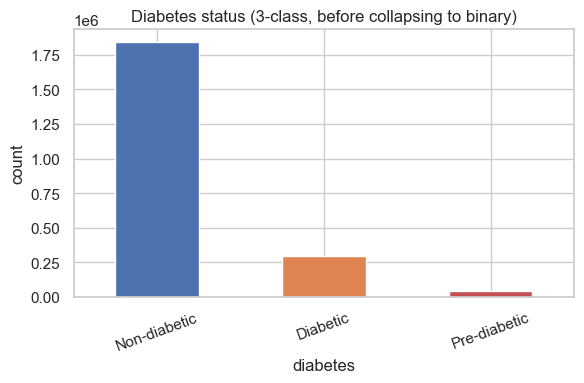
\includegraphics[width=0.55\linewidth]{images/diabetes_eda_target_3class.png}
\caption{Tình trạng tiểu đường, ba lớp gốc, trước khi gộp thành nhị phân.
Cả nhóm tiểu đường và tiền tiểu đường đều là thiểu số nhỏ so với nhóm không
tiểu đường.}
\label{fig:diabetes-eda-target}
\end{figure}

\subsection{Tìm hiểu và làm sạch dữ liệu}

BRFSS dùng các mã sentinel (mã đại diện) cho "không biết" hoặc "từ chối trả
lời" thay vì để ô trống, và những mã này có thể nằm rất xa ngoài phạm vi
của một câu trả lời thật. \verb|weight_00| có một đỉnh tăng vọt đúng tại
999 pound — một cân nặng thực tế gần như không thể có và là một giá trị
tròn, nằm ngoài phạm vi, khó có thể xảy ra ngẫu nhiên trong dữ liệu thật —
nên mọi dòng có \verb|weight_00 == 999| (chính xác là 153.060 dòng) được
gán thành missing thay vì giữ như một số đo thật. Lý luận tương tự áp dụng
cho \verb|bmi_00 > 100| (174.083 dòng), một chỉ số khối cơ thể phi thực tế
về mặt sinh lý. Cả hai giá trị sentinel này được chuyển thành missing
\textbf{trước} khi chia train/test, còn việc điền giá trị trung vị thực sự
được hoãn lại đến \textbf{sau} khi chia, để giá trị điền vào chỉ được học
từ dữ liệu train.

Việc thiếu dữ liệu ở những nơi khác trong tập dữ liệu có lời giải thích đời
thường hơn: \verb|avg_drinks_p_day_00| bị thiếu ở 52,5\% người trả lời và
\verb|poor_health_days_00| bị thiếu ở 48,6\%, cả hai đều là câu hỏi có điều
kiện trong bảng hỏi BRFSS (số ly uống trung bình mỗi ngày chỉ có ý nghĩa
khi hỏi người đã nói là có uống rượu), nên việc thiếu dữ liệu phản ánh
\textbf{thiết kế bảng hỏi}, không phải vấn đề chất lượng dữ liệu.
\verb|income_00| bị thiếu ở 17,8\% người trả lời, một mẫu hình phổ biến với
các câu hỏi về thu nhập trong khảo sát.

Một số cột hóa ra là bản sao dạng chuỗi của một cột số thứ tự (ordinal) đã
có sẵn và sạch ở nơi khác trong bảng (\verb|age_group_00| bên cạnh
\verb|age_00|, \verb|education_level_00| bên cạnh \verb|education_00|,
\verb|income_level_00| bên cạnh \verb|income_00|, \verb|general_health_00|
bên cạnh \verb|gen_health_00|, \verb|last_checkup_00| bên cạnh
\verb|l_checkup_00|); giữ cả hai sẽ hoặc đếm trùng cùng một tín hiệu hoặc
phải mã hóa lại bản chuỗi từ đầu mà không có lợi ích gì thêm, nên năm cột
chuỗi trùng lặp này bị loại bỏ và giữ lại phiên bản số thứ tự.

Phân tích khám phá dữ liệu (EDA) xác nhận các mối quan hệ lâm sàng mà mô
hình được kỳ vọng sẽ học được. BMI trung vị tăng dần từ nhóm không tiểu
đường, đến tiền tiểu đường, rồi đến tiểu đường (Hình
\ref{fig:diabetes-eda-bmi}), khớp với mối liên hệ đã được xác lập giữa cân
nặng dư thừa và nguy cơ tiểu đường type 2. Sức khỏe tự đánh giá di chuyển
gần như đơn điệu theo tình trạng tiểu đường (Hình
\ref{fig:diabetes-eda-genhealth}): người tự đánh giá sức khỏe "xuất sắc"
báo cáo tỷ lệ tiểu đường/tiền tiểu đường thấp hơn nhiều so với người tự
đánh giá "kém" — đây cũng là lý do trường thứ tự này được giữ dưới dạng mã
số thay vì one-hot encode, vì bản thân thứ tự mang thông tin. Tỷ lệ tiền
tiểu đường/tiểu đường theo năm khảo sát (Hình \ref{fig:diabetes-eda-year})
dao động nhẹ qua năm năm, từ 15,20\% (2020) đến 15,97\% (2018) — khoảng
chênh lệch quá nhỏ để tự nó biện minh mạnh mẽ cho việc giữ \verb|year| làm
đặc trưng, nhưng vẫn được giữ lại vì đây là một trong số ít tín hiệu còn
sót lại mang thông tin dư của từng đợt khảo sát, sau khi \verb|high_bp_00|
và \verb|high_cholesterol_00| đã phải bị loại bỏ do lệch schema như mô tả
ở Mục \ref{sec:diabetes}.

\begin{figure}[H]
\centering
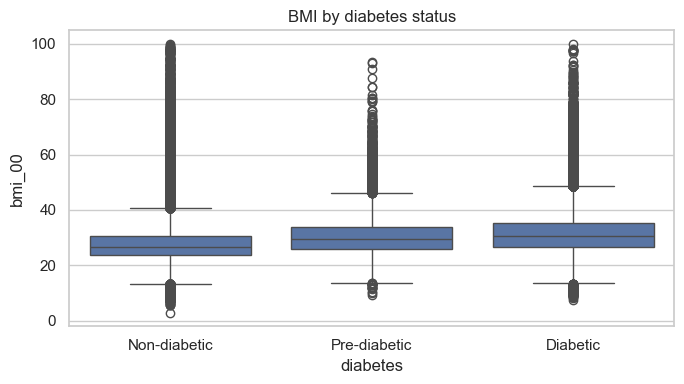
\includegraphics[width=0.55\linewidth]{images/diabetes_eda_bmi.png}
\caption{BMI theo tình trạng tiểu đường. BMI trung vị tăng dần từng bước
từ không tiểu đường, đến tiền tiểu đường, đến tiểu đường.}
\label{fig:diabetes-eda-bmi}
\end{figure}

\begin{figure}[H]
\centering
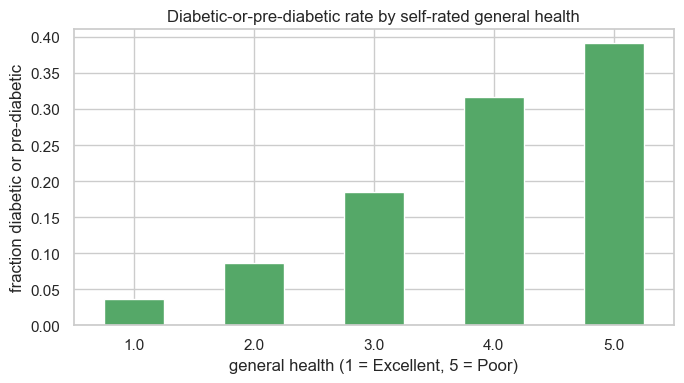
\includegraphics[width=0.55\linewidth]{images/diabetes_eda_genhealth.png}
\caption{Tỷ lệ tiền tiểu đường/tiểu đường theo sức khỏe tự đánh giá (1 =
Xuất sắc đến 5 = Kém). Tỷ lệ tăng đều từ Xuất sắc đến Kém.}
\label{fig:diabetes-eda-genhealth}
\end{figure}

\begin{figure}[H]
\centering
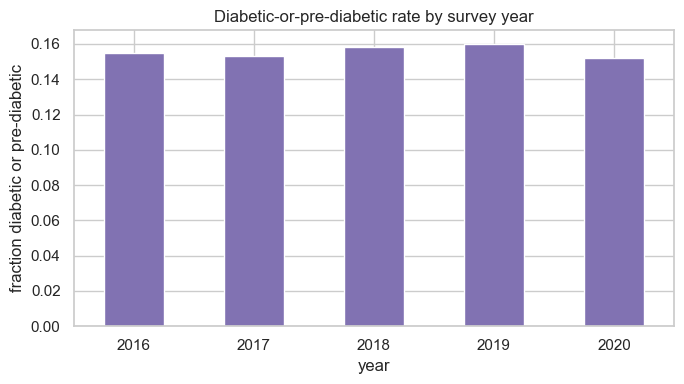
\includegraphics[width=0.55\linewidth]{images/diabetes_eda_year.png}
\caption{Tỷ lệ tiền tiểu đường/tiểu đường theo năm khảo sát, 2016-2020. Tỷ
lệ dao động nhẹ thay vì đứng yên, đây là lý do \code{year} được giữ làm
đặc trưng thay vì bị loại bỏ.}
\label{fig:diabetes-eda-year}
\end{figure}

\subsection{Biểu diễn dữ liệu}

Các cột còn lại chia thành ba nhóm, mỗi nhóm cần một cách xử lý khác nhau
trước khi mạng nơ-ron có thể sử dụng. Tám cột thực sự chỉ có hai giá trị
(giới tính, tập thể dục, tiền sử hút thuốc, sử dụng rượu, tiền sử đột quỵ,
nhồi máu cơ tim hoặc bệnh mạch vành, rào cản chi phí khám chữa bệnh) được
map trực tiếp sang 0/1 mà không mất thông tin. Bốn cột phân loại thực sự
không có thứ tự (chủng tộc, tình trạng hôn nhân, tình trạng việc làm, khả
năng tiếp cận bác sĩ riêng) được one-hot encode, vì biến "Đã kết hôn" thành
một số thứ tự đơn lẻ sẽ ngụ ý một thứ tự giữa các tình trạng hôn nhân mà
thực tế không tồn tại; việc này tạo ra 29 cột one-hot. 13 cột số còn lại —
các mã khảo sát thứ tự (sức khỏe tổng quát, trình độ học vấn) cùng với các
số đo thực sự liên tục (BMI, cân nặng, chiều cao) và bản thân \verb|year| —
tất cả được đưa vào một nhóm chuẩn hóa \code{StandardScaler}, được fit
\textbf{chỉ trên tập train}.

\verb|year| được cố tình đưa vào nhóm số được chuẩn hóa này thay vì để
nguyên dạng số nguyên lịch. Nếu không chuẩn hóa, \verb|year| (2016 đến
2020) sẽ nằm ở một thang giá trị lớn hơn nhiều lần so với mọi đặc trưng
khác, lấn át tổng có trọng số của layer đầu tiên trước khi việc huấn luyện
có cơ hội thực sự học được điều gì tốt hơn việc luôn dự đoán lớp đa số.
Chuẩn hóa nó cùng với các cột số khác loại bỏ rủi ro đó mà không làm mất đi
bất kỳ tín hiệu dư nào của đợt khảo sát mà nó mang theo.

Kết quả tạo ra một ma trận đặc trưng có độ rộng \textbf{50} (8 nhị phân $+$
29 one-hot $+$ 13 số đã chuẩn hóa). Cách chia stratified 80/20
(\code{RANDOM\_SEED = 42}) cho ra 1.744.900 dòng train và 436.225 dòng
test, với tỷ lệ dương tính 15,56\% được giữ nguyên ở cả hai tập.

Vì nhãn mục tiêu bị mất cân bằng, một lần fit thông thường sẽ được huấn
luyện để tối thiểu hóa một loss trung bình bị chi phối gần như hoàn toàn
bởi lớp đa số. Trọng số mẫu cân bằng (balanced sample weights),
$w = n_{\text{total}} / (2 \times n_{\text{class}})$, cho ra
$w_{\text{neg}} = 0.5922$ và $w_{\text{pos}} = 3.2126$, nghĩa là một sai
lầm trên một dòng tiểu đường "đắt" hơn khoảng 5,4 lần trong hàm mục tiêu
huấn luyện so với một sai lầm trên một dòng không tiểu đường. Cả ba cách
cài đặt đều áp dụng cùng cách cân bằng trọng số này, tuy nhiên, như Mục
\ref{sec:diabetes-compare} sẽ chỉ ra, \textbf{không phải qua cùng một cơ
chế} dù mang cùng một cái tên.

\subsection{Kiến trúc chung}

Cả ba cách cài đặt xây dựng cùng một mạng, được tính toán tại thời điểm
chạy dựa trên độ rộng đầu vào đã xác nhận $d = 50$ thay vì hard-code cứng:
\[
50 \to \text{Linear}(32) \to \text{ReLU} \to \text{Linear}(16) \to \text{ReLU}
\to \text{Linear}(1) \to \text{Sigmoid}
\]
với dấu vết hình dạng (shape trace), cho một batch kích thước $B$:
\[
(B, 50) \to (B, 32) \to (B, 32) \to (B, 16) \to (B, 16) \to (B, 1) \to (B, 1)
\]
Kích thước batch 2048, 25 epoch, tốc độ học 0.1, và SGD thuần túy (không
momentum, không Adam) được cố định một lần ở đây và tái sử dụng không đổi
bởi cả ba cách cài đặt, để quy tắc cập nhật của optimizer giống hệt nhau ở
cả ba, thay vì phải tự viết một bản Adam từ đầu chỉ để giữ sự công bằng
trong so sánh.

\subsection{Ba cách cài đặt}

\subsubsection{Viết tay, chỉ dùng NumPy}

Mọi thành phần là một hàm Python tường minh: \code{relu()}, một hàm
\code{binary\_cross\_entropy(y\_true, y\_pred, weights=None)} viết tay chấp
nhận trọng số cân bằng theo từng dòng, các ma trận trọng số khởi tạo bằng
He (\code{init\_params}), một hàm \code{forward} tường minh nối hai khối
\code{Linear + ReLU} rồi đến một \code{Linear + Sigmoid} cuối cùng, và một
lượt \code{backward} suy ra từng gradient bằng quy tắc chuỗi (chain rule),
với trọng số mẫu cân bằng được nhân vào tín hiệu lỗi của layer đầu ra
$dZ_3 = (A_3 - y) \odot w$ để việc hiệu chỉnh mất cân bằng lan truyền đúng
qua mọi gradient ở các layer phía sau. Một phép kiểm tra gradient bằng số
(numerical gradient check) xác nhận lượt backward tự suy ra bằng tay so
với một xấp xỉ sai phân hữu hạn (finite-difference), trước khi chạy huấn
luyện đầy đủ. Gradient descent theo mini-batch (kích thước batch 2048)
huấn luyện trong 25 epoch, mỗi batch một lượt forward, một lượt backward,
một lần cập nhật tham số.

\subsubsection{TensorFlow/Keras}

Cùng một kiến trúc trở thành một định nghĩa \code{Sequential} năm dòng
(\code{Dense(32, "relu")}, \code{Dense(16, "relu")}, \code{Dense(1,
"sigmoid")}), được compile với \code{SGD(learning\_rate=0.1)} và loss
\code{"binary\_crossentropy"}, và được huấn luyện bằng một lệnh gọi duy
nhất \code{model.fit(..., class\_weight=\{0: 0.5922, 1: 3.2126\})}.
\code{class\_weight} chính là cơ chế của Keras cho cùng việc cân bằng
trọng số đã làm bằng tay ở scratch: nó nhân đóng góp của mỗi lớp vào loss
bằng đúng các giá trị \verb|weight_neg|/\verb|weight_pos|, nên cách cài
đặt này huấn luyện trên cùng một bài toán đã được cân bằng lại về mặt hiệu
quả giống như scratch, chứ không phải một phiên bản không trọng số thông
thường. \code{model.summary()} báo cáo 2.177 tham số, khớp chính xác với
số tham số của scratch và được xác nhận bằng một phép \code{assert} trực
tiếp trong notebook.

\subsubsection{PyTorch}

Cùng kiến trúc trở thành một \code{nn.Module} (\code{DiabetesMLP}) mà
\code{forward} nối ba lớp \code{nn.Linear} với \code{nn.ReLU} xen giữa,
trả về logit thô mà không áp dụng sigmoid bên trong module.
\code{nn.BCEWithLogitsLoss(pos\_weight=...)} áp dụng sigmoid và loss
cross-entropy cùng nhau trong một bước ổn định về mặt số học, thay vì tính
riêng như scratch và Keras vẫn làm, đúng theo hướng dẫn của bài giảng là
để hàm loss hợp nhất (fused) của framework tự xử lý activation bên trong.
\code{pos\_weight} được đặt bằng
$w_{\text{pos}} / w_{\text{neg}} \approx 5.42$ — cơ chế cân bằng trọng số
riêng của PyTorch — áp dụng cho vòng lặp huấn luyện như một chu trình tường
minh \code{zero\_grad} $\to$ forward $\to$ \code{loss.backward()} $\to$
\code{optimizer.step()} thay vì một lệnh gọi \code{fit()} duy nhất.
\code{torch.optim.SGD} với cùng tốc độ học khép lại vòng lặp. Số tham số
kết quả, 2.177, khớp chính xác với cả hai cách cài đặt còn lại.

\subsection{Bảng đối chiếu thành phần theo từng cách cài đặt}

\begin{table}[H]
\centering
\caption{Diabetes: bảng đối chiếu thành phần theo từng cách cài đặt}
\footnotesize
\begin{tabular}{@{}p{2.5cm}p{4.1cm}p{4.1cm}p{4.1cm}@{}}
\toprule
Thành phần & Scratch & Keras & PyTorch \\
\midrule
Tải dữ liệu & \code{pandas.read\_csv} $\times5$, \code{pd.concat} & giống nhau & giống nhau \\
Tiền xử lý & chuẩn hóa mean/std viết tay & tương đương StandardScaler (viết tay, dùng chung) & giống scratch \\
Định nghĩa mô hình & các hàm tường minh $+$ một dict tham số & \code{Sequential([...])} & lớp con \code{nn.Module} \\
Activation & \code{relu()}, \code{sigmoid()} & \code{activation="relu"/"sigmoid"} & \code{nn.ReLU()}, hợp nhất trong \code{BCEWithLogitsLoss} \\
Lớp Dense/Linear & \code{linear()} (matmul thủ công) & \code{Dense(...)} & \code{nn.Linear(...)} \\
Loss & \code{binary\_cross\_entropy} viết tay & \code{"binary\_crossentropy"} & \code{nn.BCEWithLogitsLoss()} \\
Gradient & backprop viết tay & autodiff (ngầm định trong \code{fit}) & \code{loss.backward()} (autograd) \\
Optimizer & \code{W -= lr * dW} viết tay & \code{optimizer="sgd"} & \code{torch.optim.SGD(...)} \\
Vòng lặp huấn luyện & \code{for epoch / for batch} tường minh & \code{model.fit(...)} & \code{for epoch / for batch} tường minh \\
Đánh giá & các hàm đo chỉ số viết tay & tương đương \code{model.evaluate} (viết tay) & viết tay (\code{model.eval()}, no-grad) \\
Dự đoán & \code{forward(X\_test, params)} & \code{model.predict(...)} & \code{model(x\_test)} trong \code{torch.no\_grad()} \\
\bottomrule
\end{tabular}
\end{table}

\subsection{Đường cong huấn luyện và đánh giá}

\begin{figure}[H]
\centering
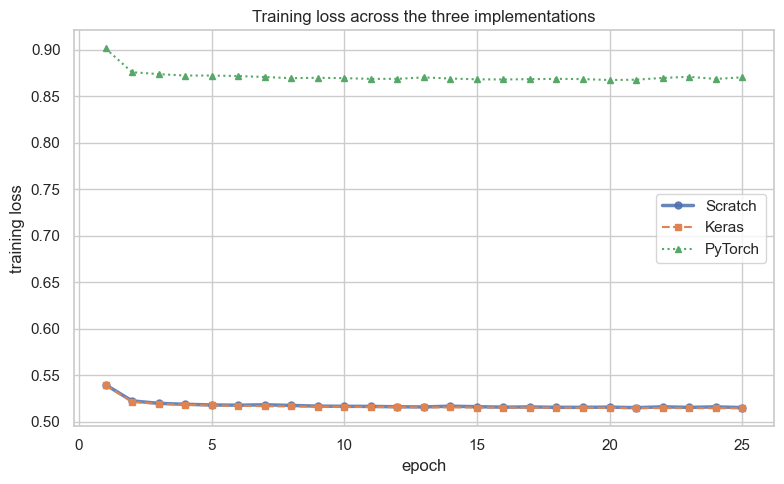
\includegraphics[width=\linewidth]{images/diabetes_compare_loss.png}
\caption{Loss huấn luyện của ba cách cài đặt, mỗi đường một cách cài đặt.
Scratch và Keras bám sát nhau; đường của PyTorch nằm trên một thang giá
trị số rõ ràng khác biệt, lý do được giải thích ở Mục
\ref{sec:diabetes-compare}.}
\end{figure}

\begin{figure}[H]
\centering
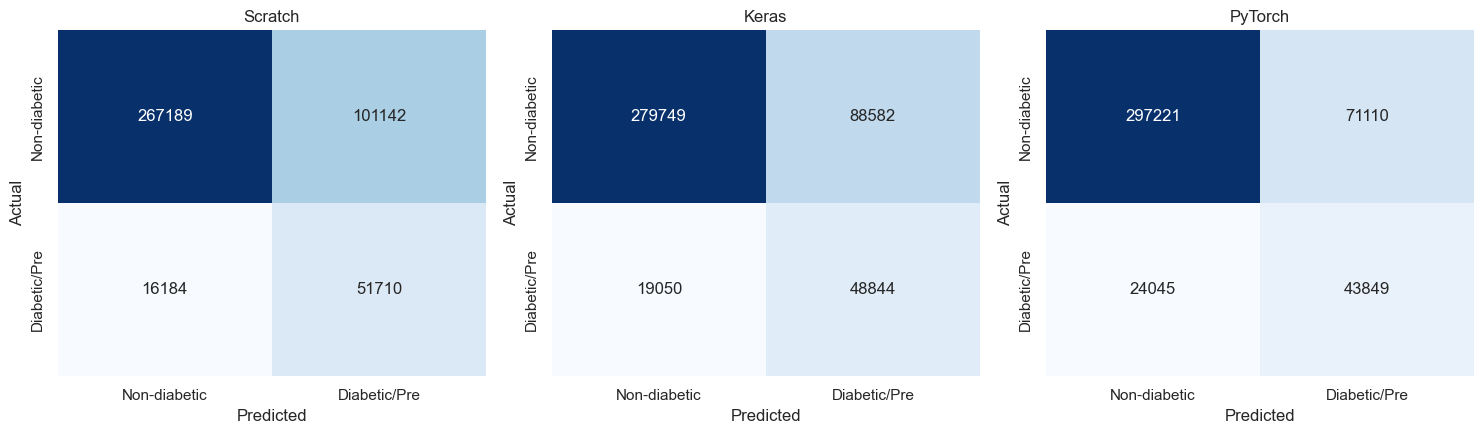
\includegraphics[width=\linewidth]{images/diabetes_compare_confmat.png}
\caption{Ma trận nhầm lẫn (confusion matrix) của ba cách cài đặt trên tập
test Diabetes (436.225 dòng).}
\end{figure}

\begin{table}[H]
\centering
\caption{Diabetes: so sánh định lượng, tập test}
\label{tab:diabetes-quant}
\begin{tabular}{lrrrrrr}
\toprule
Cách cài đặt & Tham số & T.gian train (s) & Loss cuối & Accuracy & Precision & Recall \\
\midrule
Scratch & 2.177 & 69.4 & 0.5155 & 0.7310 & 0.3383 & 0.7616 \\
Keras & 2.177 & 24.7 & 0.5148 & 0.7533 & 0.3554 & 0.7194 \\
PyTorch & 2.177 & 311.0 & 0.8706 & 0.7819 & 0.3814 & 0.6458 \\
\bottomrule
\end{tabular}
\end{table}

F1 cho cùng ba cách cài đặt, theo đúng thứ tự: 0.4685 (scratch), 0.4758
(Keras), 0.4796 (PyTorch).

\begin{figure}[H]
\centering

\includegraphics[width=0.6\linewidth]{images/diabetes_compare_accuracy.png}
\caption{Độ chính xác trên tập test theo từng cách cài đặt.}
\end{figure}

\begin{figure}[H]
\centering

\includegraphics[width=0.7\linewidth]{images/diabetes_compare_prf1.png}
\caption{Precision, recall, và F1 theo từng cách cài đặt. Cả ba đều nằm
trong khoảng precision 0.34-0.38, recall 0.65-0.76 — dấu vết đặc trưng của
việc cân bằng trọng số trên một nhãn mục tiêu mất cân bằng: bắt được nhiều
hơn các trường hợp dương tính hiếm, đổi lại là nhiều dự đoán dương tính
sai hơn.}
\end{figure}

\begin{figure}[H]
\centering
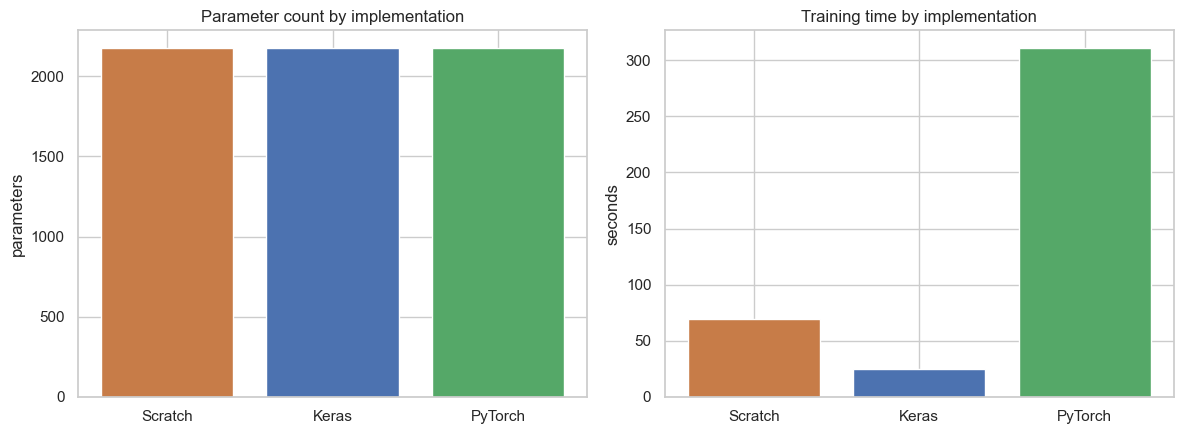
\includegraphics[width=\linewidth]{images/diabetes_compare_params_time.png}
\caption{Số lượng tham số (giống hệt nhau ở cả ba, xác nhận cùng kiến
trúc) và thời gian huấn luyện theo từng cách cài đặt.}
\end{figure}

\subsection{Thảo luận so sánh}
\label{sec:diabetes-compare}

Về accuracy và F1, PyTorch về đích nhỉnh hơn một chút (0.782, 0.480), Keras
theo sát phía sau (0.753, 0.476), và scratch lùi thêm một bước nhỏ tương tự
(0.731, 0.469). Cả ba nằm trong khoảng chênh lệch khoảng năm điểm phần
trăm với nhau ở cả hai chỉ số — đây chính là điều nên xảy ra khi cùng một
kiến trúc được huấn luyện trên cùng dữ liệu với cùng siêu tham số ba lần
riêng biệt: một khoảng cách cỡ này dễ dàng quy về các chi tiết cấp độ
framework, độ chính xác số học mặc định, cách mỗi framework xáo trộn
(shuffle) batch của nó, những khác biệt nhỏ trong cách áp dụng cân bằng
trọng số — chứ không phải do một cách cài đặt nào đó thực sự học được một
mô hình tốt hơn có ý nghĩa.

Có một con số trong Bảng \ref{tab:diabetes-quant} thực sự \textbf{không thể
so sánh trực tiếp} giữa các cách cài đặt, và đáng để giải thích thay vì lướt
qua: loss huấn luyện cuối cùng. Scratch và Keras đều ở quanh mức 0.51,
trong khi PyTorch ở mức 0.87 — một chênh lệch lớn hơn nhiều so với những
gì khoảng cách accuracy gợi ý. Khoảng cách này đến hoàn toàn từ cách mỗi
cách cài đặt áp dụng cân bằng trọng số lớp, chứ không phải do PyTorch huấn
luyện tệ hơn. Cả scratch và Keras đều scale loss của \textit{mọi} dòng,
nhân các dòng lớp âm với $w_{\text{neg}} = 0.5922$ và các dòng lớp dương
với $w_{\text{pos}} = 3.2126$, giữ loss ở gần đúng thang giá trị mà một
loss không trọng số sẽ có. \code{BCEWithLogitsLoss(pos\_weight=...)} của
PyTorch chỉ scale số hạng của lớp dương, theo tỉ lệ
$w_{\text{pos}} / w_{\text{neg}} \approx 5.42$, để số hạng lớp âm không bị
scale. Đây là một cách hợp lệ và phổ biến để áp dụng cân bằng trọng số lớp
trong PyTorch, nhưng nó tạo ra một giá trị loss trên một thang khác, không
phải một con số so sánh trực tiếp được. Đây chính xác là loại chi tiết cấp
độ cài đặt mà bài tập này được thiết kế để phơi bày: ba framework cùng
cung cấp "cùng một" tính năng cân bằng trọng số lớp dưới những cái tên gợi
ý sự tương đương (\code{class\_weight}, một tham số \code{weights},
\code{pos\_weight}), nhưng thực tế tham số hóa nó khác nhau bên dưới.

Thời gian huấn luyện kể một câu chuyện khác với accuracy. Keras nhanh nhất
(24.7s), scratch đứng kế tiếp (69.4s), và PyTorch chậm hơn rõ rệt (311.0s),
gần gấp bốn lần rưỡi thời gian của scratch cho một mạng chỉ có 2.177 tham
số. Điều này khớp với cách mỗi cách cài đặt tiêu tốn thời gian: \code{fit()}
của Keras chạy vòng lặp huấn luyện trong một đồ thị đã biên dịch với rất ít
overhead Python trên mỗi batch; vòng lặp mini-batch của scratch là Python
thuần, nhưng mỗi batch chỉ làm một vài phép nhân ma trận trên một mạng rất
nhỏ, nên bản thân các lệnh gọi NumPy chiếm ưu thế hơn overhead của vòng
lặp; vòng lặp theo từng batch của PyTorch bao gồm việc xây dựng và tháo dỡ
đồ thị autograd ở mỗi bước, một chi phí gần như cố định trên mỗi batch mà
quan trọng hơn nhiều đối với một mạng nhỏ như thế này so với một mạng lớn
hơn — nơi phần tính toán thực sự mới là yếu tố chiếm ưu thế. Sự linh hoạt
của PyTorch — một vòng lặp huấn luyện tường minh, có thể kiểm tra được,
cùng với autograd — đi kèm một overhead thực sự trên mỗi bước mà một mạng
kích thước này không thể khấu hao hết, một sự đánh đổi sẽ trông rất khác
một khi có convolution thực sự xuất hiện ở các Mục \ref{sec:fashion} và
\ref{sec:cifar10}.

Framework nào ẩn nhiều nhất, và framework nào cho quyền kiểm soát nhiều
nhất: Keras cũng ẩn gần như mọi thứ ở đây — việc tính loss, cơ chế cân bằng
trọng số lớp, lượt backward, và vòng lặp huấn luyện đều gói gọn trong một
lệnh gọi \code{compile()} và một lệnh gọi \code{fit()}. PyTorch chỉ ẩn lượt
backward, giữ vòng lặp huấn luyện và cơ chế trọng số loss ở dạng tường
minh, và chính sự tường minh đó là thứ đã phơi bày sự bất đối xứng của
\code{pos\_weight} ở trên — một chi tiết đáng lẽ sẽ vô hình bên trong một
lệnh gọi \code{fit()} đóng gói. Scratch không ẩn gì cả, đổi lại là cái giá
trực tiếp: cách cài đặt tốn nhiều code nhất để viết và debug.

\newpage
% ---------------------------------------------------------------------
\section{Fashion-MNIST: Phân loại ảnh 10 lớp (CNN)}
\label{sec:fashion}
% ---------------------------------------------------------------------

\subsection{Mô tả bài toán}

Ứng dụng này phân loại một ảnh xám $28\times28$ của một món trang phục vào
một trong mười loại (áo phông/áo thun, quần dài, áo len chui đầu, đầm, áo
khoác, dép sandal, áo sơ mi, giày thể thao, túi xách, giày bốt cổ ngắn).
Khác với ứng dụng Diabetes, đầu vào ở đây có cấu trúc không gian 2 chiều
thực sự — các pixel liền kề có liên quan với nhau, và một hình dạng như
tay áo hay đế giày là một pattern cục bộ lặp lại ở nhiều vị trí khác nhau
trong ảnh — đúng bối cảnh mà Lecture 04 đưa ra để giải thích tại sao CNN,
chứ không phải MLP, mới là kiến trúc phù hợp: kết nối cục bộ (local
connectivity) và chia sẻ trọng số (weight sharing) cho phép một tập nhỏ
các kernel đã học phát hiện cùng một pattern ở bất cứ đâu trong ảnh.

\subsection{Tập dữ liệu}

Fashion-MNIST được tải qua
\code{keras.datasets.fashion\_mnist.load\_data()}, tự động tải và cache dữ
liệu ngay lần dùng đầu tiên, không cần quản lý file thủ công. Bộ dữ liệu
gồm 60.000 ảnh train và 10.000 ảnh test, mỗi ảnh $28\times28$ pixel, một
kênh màu, giá trị pixel trong $[0, 255]$ trước khi chuẩn hóa. Mỗi lớp
trong mười lớp có đúng 6.000 ảnh train và 1.000 ảnh test (Hình
\ref{fig:fm-eda-balance}) — một benchmark được cố tình cân bằng, nên không
cần hiệu chỉnh mất cân bằng lớp ở đây, khác với ứng dụng Diabetes: một mô
hình luôn dự đoán một lớp duy nhất sẽ chỉ đạt 10\% accuracy, chứ không phải
một con số cao đánh lừa như trên một nhãn mục tiêu mất cân bằng.

\begin{figure}[H]
\centering
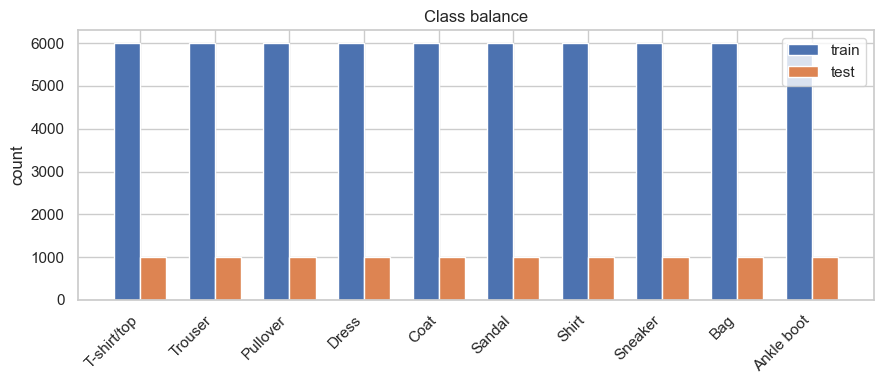
\includegraphics[width=0.7\linewidth]{images/fashion_mnist_eda_class_balance.png}
\caption{Cân bằng lớp của Fashion-MNIST, tập train và test. Mỗi lớp có
đúng 6.000 ảnh train và 1.000 ảnh test.}
\label{fig:fm-eda-balance}
\end{figure}

\begin{figure}[H]
\centering
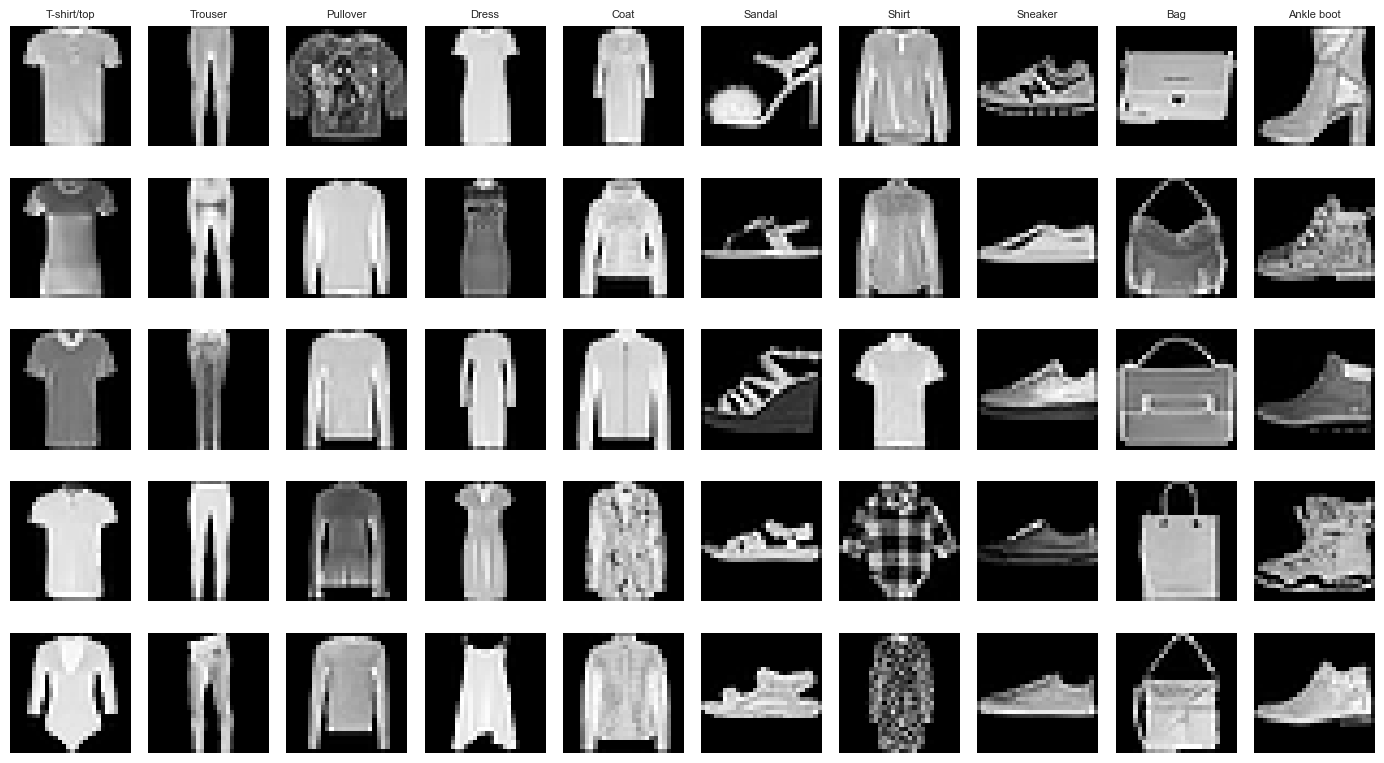
\includegraphics[width=\linewidth]{images/fashion_mnist_eda_sample_grid.png}
\caption{Năm ảnh mẫu cho mỗi lớp. Các lớp phân biệt rõ ràng ở những trường
hợp hiển nhiên và thực sự giống nhau ở một số trường hợp khác (áo sơ mi vs.
áo len chui đầu vs. áo khoác), đây là một nguồn hợp lý của các lỗi phân
loại thấy được ở phần sau.}
\end{figure}

\begin{figure}[H]
\centering
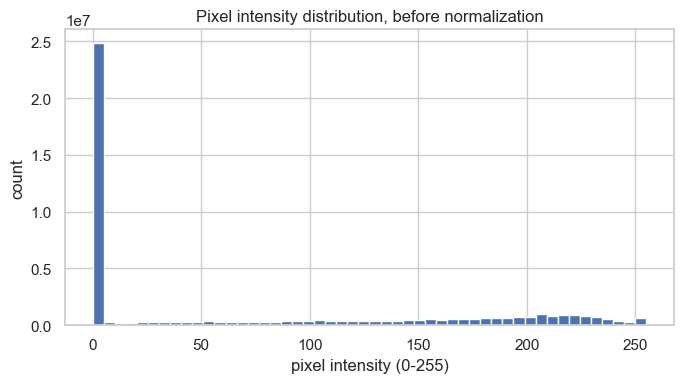
\includegraphics[width=0.6\linewidth]{images/fashion_mnist_eda_pixel_hist.png}
\caption{Phân bố cường độ pixel trước khi chuẩn hóa. Đỉnh lớn tại 0 phản
ánh việc phần lớn mỗi ảnh là nền đen trơn xung quanh món trang phục được
căn giữa.}
\end{figure}

\subsection{Biểu diễn dữ liệu}

Giá trị pixel được ép kiểu \code{float32} và chia cho 255, ánh xạ khoảng
số nguyên $[0,255]$ sang $[0,1]$. Hai cách sắp xếp mảng được giữ song song
cho phần còn lại của notebook: channel-first, $(N, 1, 28, 28)$, cho scratch
và PyTorch, và channel-last, $(N, 28, 28, 1)$, cho layout convolution mặc
định của Keras. Không cần làm sạch thêm, vì đây là một benchmark dataset
đã được tuyển chọn, không có giá trị thiếu, không có mã sentinel, và không
có sự không nhất quán về schema cần xử lý.

\subsection{Kiến trúc chung}

Cả ba cách cài đặt xây dựng cùng một mạng:
\[
\resizebox{\linewidth}{!}{$28\times28\times1 \to \text{Conv}(1{\to}32, k{=}3, \text{pad}{=}1) \to \text{ReLU}
\to \text{MaxPool}(2) \to \text{Conv}(32{\to}64, k{=}3, \text{pad}{=}1) \to
\text{ReLU} \to \text{MaxPool}(2)$}
\]
\[
\to \text{Flatten} (64{\times}7{\times}7 = 3136) \to \text{Linear}(3136{\to}128)
\to \text{ReLU} \to \text{Linear}(128{\to}10)
\]
với dấu vết hình dạng, cho một batch kích thước $B$:
\[
\resizebox{\linewidth}{!}{$(B,1,28,28) \to (B,32,28,28) \to (B,32,14,14) \to (B,64,14,14) \to (B,64,7,7)
\to (B,3136) \to (B,128) \to (B,10)$}
\]
Kích thước batch 256, 10 epoch, tốc độ học 0.05, và SGD thuần túy được cố
định một lần ở đây và tái sử dụng không đổi ở cả ba cách cài đặt.

\subsection{Ba cách cài đặt}

\subsubsection{Viết tay, chỉ dùng NumPy}

Mọi phép toán — convolution, pooling, các lớp dense, loss, và mọi gradient
— đều được cài đặt bằng tay. Convolution là phép toán đáng để nói cụ thể:
một kernel $3\times3$ được đặt chồng lên một patch ảnh $3\times3$, chín cặp
(giá trị kernel, pixel) chồng lấn được nhân và cộng thành một giá trị đầu
ra, và kernel trượt qua mọi vị trí để xây dựng toàn bộ feature map — cùng
một kernel được tái sử dụng ở mọi vị trí, tức chia sẻ trọng số (weight
sharing), chính là cái cho phép một kernel nhỏ tổng quát hóa trên toàn bộ
ảnh thay vì chỉ nhận ra một pattern ở đúng vị trí nó từng được huấn luyện.
Một vòng lặp trực tiếp theo từng vị trí thực hiện phép toán này chậm đến
mức không khả thi — riêng lớp convolution thứ hai đã mất hơn hai giây mỗi
batch với kích thước layer thực tế của mạng này — nên
\code{conv2d\_forward}/\code{conv2d\_backward} của notebook thay vào đó
dùng phương pháp \code{im2col}: mọi patch mà kernel sẽ từng chạm tới được
trích xuất trước dưới dạng một view có sải bước (strided view) không sao
chép (zero-copy), rồi xếp chồng thành một ma trận duy nhất, biến toàn bộ
convolution thành một phép nhân ma trận duy nhất — đúng phép tính giống hệt
vòng lặp naive, nhưng thực hiện cho mọi vị trí cùng lúc thay vì từng vị trí
một, nhanh hơn khoảng 40 lần với kích thước layer thực tế của mạng này. Một
phép kiểm tra gradient bằng số xác nhận các lượt backward của convolution
và pooling tự suy ra bằng tay so với một xấp xỉ sai phân hữu hạn, trước khi
chạy huấn luyện đầy đủ; phép kiểm tra này đã bắt được một bug thật trong
quá trình phát triển — một phép chia dư $1/N$ trong lượt backward của lớp
dense đã âm thầm làm co nhỏ mọi gradient của lớp dense (các gradient của
lớp convolution, được tính bởi một nhánh code khác không có phép chia đó,
không bị ảnh hưởng) — đã được sửa trước khi các kết quả báo cáo bên dưới
được tạo ra. Gradient descent theo mini-batch (kích thước batch 256, 235
batch mỗi epoch) huấn luyện trong 10 epoch.

\subsubsection{TensorFlow/Keras}

Cùng kiến trúc trở thành một định nghĩa \code{Sequential} tám lớp
(\code{Conv2D(32,3,padding="same",activation="relu")},
\code{MaxPooling2D(2)}, \code{Conv2D(64,...)}, \code{MaxPooling2D(2)},
\code{Flatten()}, \code{Dense(128,"relu")}, \code{Dense(10)}), được compile
với \code{SGD(learning\_rate=0.05)} và
\code{SparseCategoricalCrossentropy(from\_logits=True)}, huấn luyện bằng
một lệnh gọi \code{model.fit(X\_train\_hwc, y\_train, batch\_size=256,
epochs=10)}. \code{model.summary()} báo cáo 421.642 tham số, khớp chính
xác với scratch. Các vòng lặp convolution và pooling mà scratch phải viết
tường minh đã hoàn toàn biến mất khỏi code của cách cài đặt này, được đóng
gói thay vào bên trong các đối tượng layer \code{Conv2D}/\code{MaxPooling2D}.

\subsubsection{PyTorch}

Cùng kiến trúc trở thành một \code{nn.Module} (\code{FashionCNN}) với một
khối \code{self.features} (\code{nn.Conv2d}, \code{nn.ReLU},
\code{nn.MaxPool2d}, lặp lại hai lần) theo sau bởi một khối
\code{self.classifier} (\code{nn.Flatten}, \code{nn.Linear(3136,128)},
\code{nn.ReLU}, \code{nn.Linear(128,10)}), trả về logit thô được tiêu thụ
bởi \code{nn.CrossEntropyLoss()}. Vòng lặp huấn luyện vẫn tường minh
(\code{zero\_grad} $\to$ forward $\to$ loss $\to$ \code{backward()}
$\to$ \code{optimizer.step()}), với \code{torch.optim.SGD} cùng tốc độ
học. Số tham số kết quả, 421.642, khớp chính xác với cả hai cách cài đặt
còn lại, được xác nhận bằng một phép \code{assert} trực tiếp trong notebook.

\subsection{Bảng đối chiếu thành phần theo từng cách cài đặt}

\begin{table}[H]
\centering
\caption{Fashion-MNIST: bảng đối chiếu thành phần theo từng cách cài đặt}
\footnotesize
\begin{tabular}{@{}p{2.5cm}p{4.1cm}p{4.1cm}p{4.1cm}@{}}
\toprule
Thành phần & Scratch & Keras & PyTorch \\
\midrule
Tải dữ liệu & bộ tải của Keras, mảng NumPy dùng chung & giống nhau & giống nhau \\
Tiền xử lý & /255, reshape channel-first viết tay & /255, channel-last (mặc định) & /255, channel-first \\
Định nghĩa mô hình & các hàm tường minh $+$ một dict tham số & \code{Sequential([...])} & lớp con \code{nn.Module} \\
Convolution & \code{conv2d\_forward}/\code{backward} (\code{im2col}) & \code{Conv2D(...)} & \code{nn.Conv2d(...)} \\
Activation & \code{relu()} & \code{activation="relu"} & \code{nn.ReLU()} \\
Pooling & \code{max\_pool2d\_forward}/\code{backward} & \code{MaxPooling2D(2)} & \code{nn.MaxPool2d(2)} \\
Flatten & \code{flatten\_forward}/\code{backward} (reshape) & \code{Flatten()} & \code{nn.Flatten()} \\
Lớp Dense/Linear & \code{linear\_forward}/\code{backward} & \code{Dense(...)} & \code{nn.Linear(...)} \\
Loss & softmax cross-entropy viết tay & \code{SparseCategorical}\allowbreak\code{Crossentropy(}\allowbreak\code{from\_logits=True)} & \code{nn.CrossEntropyLoss()} \\
Gradient & backprop viết tay & autodiff (ngầm định trong \code{fit}) & \code{loss.backward()} (autograd) \\
Optimizer & \code{W -= lr * dW} viết tay & \code{optimizer="sgd"} & \code{torch.optim.SGD(...)} \\
Vòng lặp huấn luyện & \code{for epoch / for batch} tường minh & \code{model.fit(...)} & \code{for epoch / for batch} tường minh \\
Đánh giá & các hàm đo chỉ số viết tay & tương đương \code{model.evaluate} (viết tay) & viết tay (\code{model.eval()}, no-grad) \\
Dự đoán & \code{forward(X\_test, params)} & \code{model.predict(...)} & \code{model(x\_test)} trong \code{torch.no\_grad()} \\
\bottomrule
\end{tabular}
\end{table}

\subsection{Đường cong huấn luyện và đánh giá}

\begin{figure}[H]
\centering
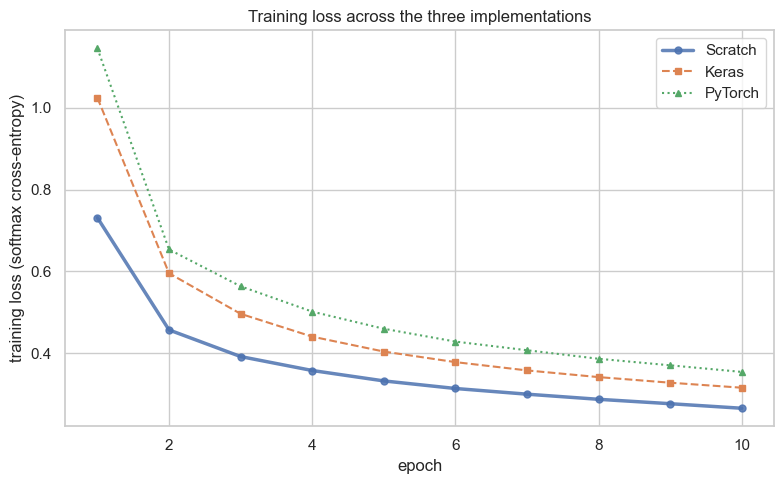
\includegraphics[width=\linewidth]{images/fashion_mnist_compare_loss.png}
\caption{Loss huấn luyện của ba cách cài đặt.}
\end{figure}

\begin{figure}[H]
\centering
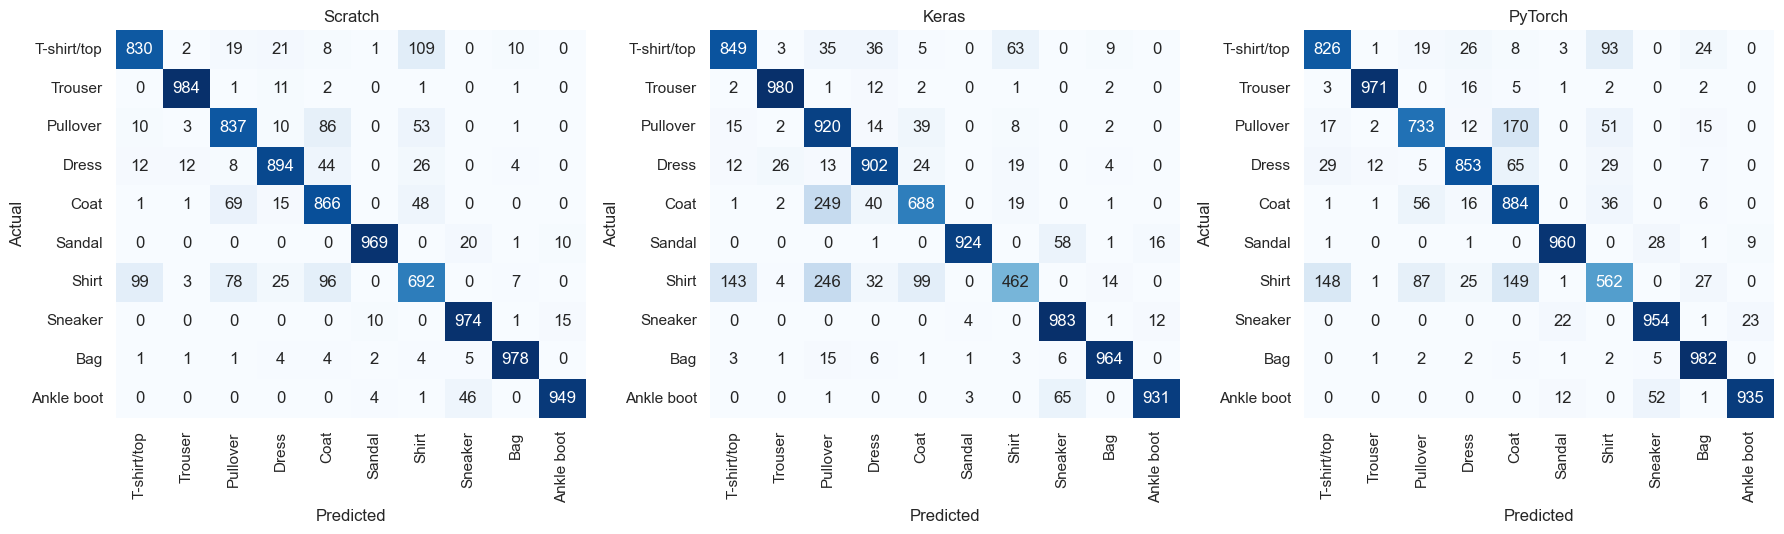
\includegraphics[width=\linewidth]{images/fashion_mnist_compare_confmat.png}
\caption{Ma trận nhầm lẫn của ba cách cài đặt trên tập test Fashion-MNIST
(10.000 ảnh). Cụm áo sơ mi/áo len chui đầu/áo khoác là nguồn nhầm lẫn phổ
biến nhất ở cả ba, khớp với mức độ giống nhau về hình ảnh giữa các lớp này
(hình bên cạnh Hình \ref{fig:fm-eda-balance}).}
\end{figure}

\begin{table}[H]
\centering
\caption{Fashion-MNIST: so sánh định lượng, tập test}
\label{tab:fm-quant}
\begin{tabular}{lrrrrrr}
\toprule
Cách cài đặt & Tham số & T.gian train (s) & Loss cuối & Accuracy & Precision (macro) & Recall (macro) \\
\midrule
Scratch & 421.642 & 1.330,5 & 0.2655 & 0.8973 & 0.8976 & 0.8973 \\
Keras & 421.642 & 75,6 & 0.3157 & 0.8603 & 0.8695 & 0.8603 \\
PyTorch & 421.642 & 191,5 & 0.3544 & 0.8660 & 0.8676 & 0.8660 \\
\bottomrule
\end{tabular}
\end{table}

F1-macro cho cùng ba cách cài đặt, theo đúng thứ tự: 0.8970 (scratch),
0.8565 (Keras), 0.8641 (PyTorch).

\begin{figure}[H]
\centering
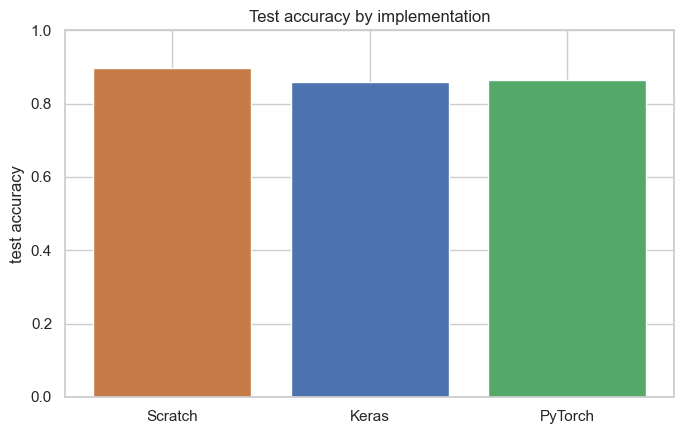
\includegraphics[width=0.6\linewidth]{images/fashion_mnist_compare_accuracy.png}
\caption{Độ chính xác trên tập test theo từng cách cài đặt. Scratch thắng
ở đây — ứng dụng duy nhất trong báo cáo này mà scratch thắng.}
\end{figure}

\begin{figure}[H]
\centering
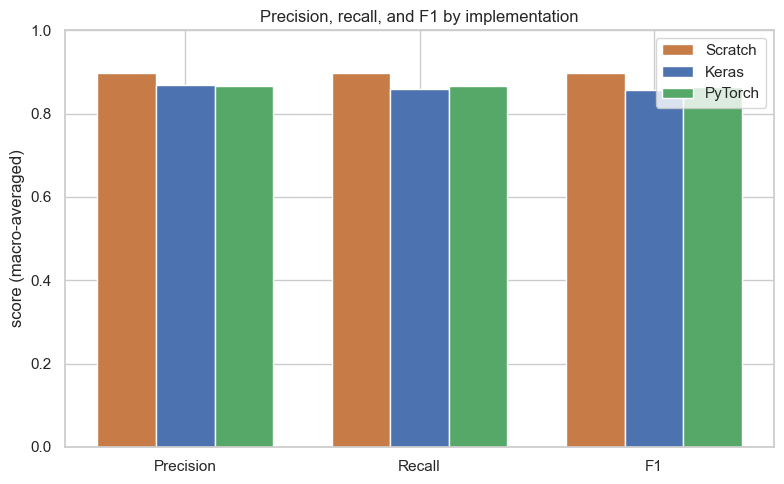
\includegraphics[width=0.7\linewidth]{images/fashion_mnist_compare_prf1.png}
\caption{Precision, recall, và F1 (trung bình macro) theo từng cách cài
đặt.}
\end{figure}

\begin{figure}[H]
\centering
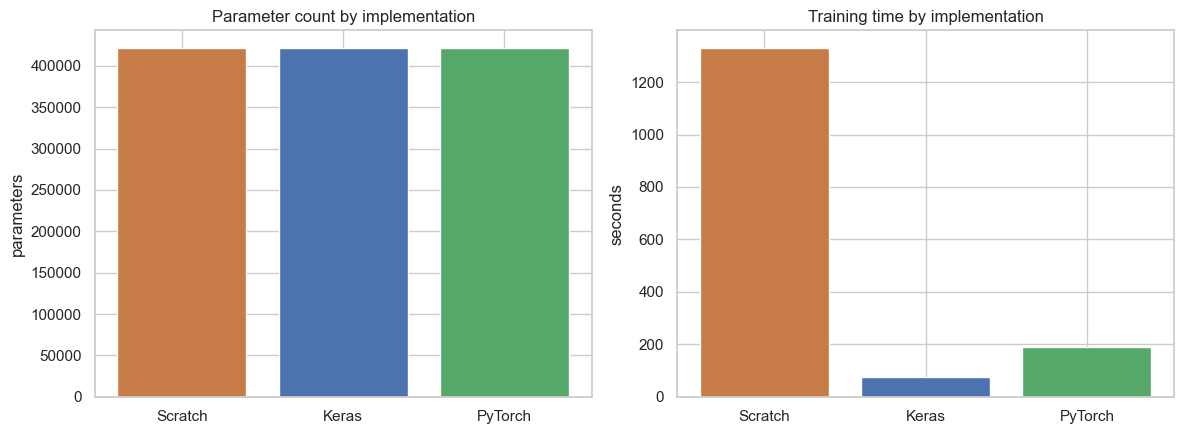
\includegraphics[width=\linewidth]{images/fashion_mnist_compare_params_time.png}
\caption{Số lượng tham số (giống hệt nhau ở cả ba) và thời gian huấn luyện
theo từng cách cài đặt. Thời gian huấn luyện của scratch nằm trên một
thang giá trị khác biệt rõ rệt so với hai cách còn lại.}
\end{figure}

\subsection{Thảo luận so sánh}
\label{sec:fm-compare}

Theo độ chính xác trên tập test, scratch thực sự vượt lên trên: 0.897 so
với 0.866 của PyTorch và 0.860 của Keras. Đây là một kết quả thực sự thú
vị, vì scratch thường không phải là cách cài đặt được kỳ vọng sẽ thắng.
Lời giải thích khả dĩ nhất là do khởi tạo và tính ngẫu nhiên, chứ không
phải do bản thân cách cài đặt tốt hơn về bản chất: scratch dùng khởi tạo
He tường minh với seed cố định, trong khi Keras và PyTorch mỗi bên áp dụng
bộ khởi tạo mặc định riêng, cũng phù hợp với ReLU nhưng không đảm bảo cho
ra cùng một điểm khởi đầu. Mười epoch không phải là nhiều huấn luyện, nên
sự khác biệt về điểm khởi đầu của mỗi cách cài đặt vẫn có thể ảnh hưởng
đáng kể đến điểm kết thúc. Cả ba đều nằm trong khoảng chênh lệch khoảng
bốn điểm phần trăm về accuracy — đủ nhỏ để phù hợp với việc đây là ba cách
cài đặt của cùng một kiến trúc, chứ không phải ba mô hình thực sự khác
nhau, tương tự độ chênh lệch đã thấy ở ứng dụng Diabetes.

Thời gian huấn luyện kể câu chuyện kịch tính hơn ở đây. Scratch mất
1.330,5 giây (khoảng 22 phút), Keras mất 75,6 giây, và PyTorch mất 191,5
giây — scratch chậm hơn Keras khoảng 17,6 lần và chậm hơn PyTorch khoảng
6,9 lần. Khoảng cách này hợp lý xét theo những gì mỗi cách cài đặt thực sự
đang làm bên dưới: \code{fit()} của Keras chạy toàn bộ vòng lặp huấn luyện
bên trong một đồ thị đã biên dịch, với convolution được cài đặt bằng các
hàm vector hóa tối ưu cao và gần như không có overhead Python trên mỗi
batch. Vòng lặp huấn luyện tường minh của PyTorch mang một chút overhead
Python và autograd trên mỗi batch, nhưng phép toán convolution của nó vẫn
là một hàm đã biên dịch, được tối ưu. \code{conv2d\_forward}/
\code{conv2d\_backward} của scratch, dù đã được tăng tốc bằng \code{im2col}
so với vòng lặp theo từng vị trí naive, vẫn chỉ là các phép nhân ma trận
NumPy thuần túy được phát ra từ một vòng lặp huấn luyện Python, không có
sự hợp nhất toán tử (operator fusion) hay tối ưu hóa cấp thấp nào mà một
framework deep learning trưởng thành áp dụng riêng cho convolution. Việc
viết lại bằng \code{im2col} giúp việc huấn luyện trở nên khả thi; nó không
thu hẹp khoảng cách với các framework được xây dựng và tối ưu chuyên biệt
cho phép toán này. Đây là một sự tương phản rõ rệt với MLP Diabetes ở Mục
\ref{sec:diabetes-compare}, nơi scratch nhanh tương đương các framework và
PyTorch thực ra là cách cài đặt chậm nhất: một khi lượt forward của mạng
thực sự liên quan đến convolution thay vì chỉ các phép nhân ma trận nhỏ ở
lớp dense, bức tranh về tốc độ đảo ngược hoàn toàn.

Framework nào ẩn nhiều nhất, và framework nào cho quyền kiểm soát nhiều
nhất: Keras ẩn gần như mọi thứ — convolution, pooling, lượt backward, và
vòng lặp huấn luyện đều gói trong một định nghĩa \code{Sequential} và một
lệnh gọi \code{fit()}. PyTorch ẩn lượt backward qua autograd nhưng giữ
vòng lặp huấn luyện và cách ghép layer ở dạng tường minh. Scratch không ẩn
gì cả, mọi phép nhân, mọi gradient, và mọi lần cập nhật tham số đều là code
được viết ra và có thể đọc từng dòng. Cái giá của sự hiển thị đó, trong
ứng dụng này, là một chênh lệch rất thực về thời gian huấn luyện thực tế
(wall-clock) — đúng sự đánh đổi mà ba mức độ trừu tượng được dùng để đại
diện: nhiều tiện lợi và tốc độ hơn đổi lấy mất khả năng hiển thị, hoặc
nhiều khả năng hiển thị và kiểm soát hơn đổi lấy mất sự tiện lợi và tốc độ.

\newpage
% ---------------------------------------------------------------------
\section{CIFAR-10: Phân loại ảnh 10 lớp (CNN)}
\label{sec:cifar10}
% ---------------------------------------------------------------------

\subsection{Mô tả bài toán}

Ứng dụng này phân loại một ảnh chụp màu RGB $32\times32$ vào một trong
mười loại vật thể (máy bay, ô tô, chim, mèo, hươu, chó, ếch, ngựa, tàu
thủy, xe tải). Ứng dụng dùng cùng họ kiến trúc với Fashion-MNIST, một CNN,
với cùng lý do — có cấu trúc không gian 2 chiều thực sự mà convolution có
thể khai thác — nhưng với ba kênh đầu vào thay vì một, và một bài toán khó
hơn đáng kể: phân biệt mèo với chó, hay ô tô với xe tải, trong một bức
ảnh chụp thật được nén xuống $32\times32$ pixel, là một bài toán thị giác
thực sự khó hơn so với phân biệt các hình dáng trang phục trên nền trơn.

\subsection{Tập dữ liệu}

CIFAR-10 được tải qua \code{keras.datasets.cifar10.load\_data()}, tự động
tải và cache dữ liệu ngay lần dùng đầu tiên ($\sim$170MB, chỉ tải một lần).
Bộ dữ liệu gồm 50.000 ảnh train và 10.000 ảnh test, mỗi ảnh $32\times32$
pixel, ba kênh màu, giá trị pixel trong $[0,255]$ trước khi chuẩn hóa. Mỗi
lớp trong mười lớp có đúng 5.000 ảnh train và 1.000 ảnh test — một
benchmark khác được cố tình cân bằng, không cần hiệu chỉnh trọng số lớp.

\begin{figure}[H]
\centering
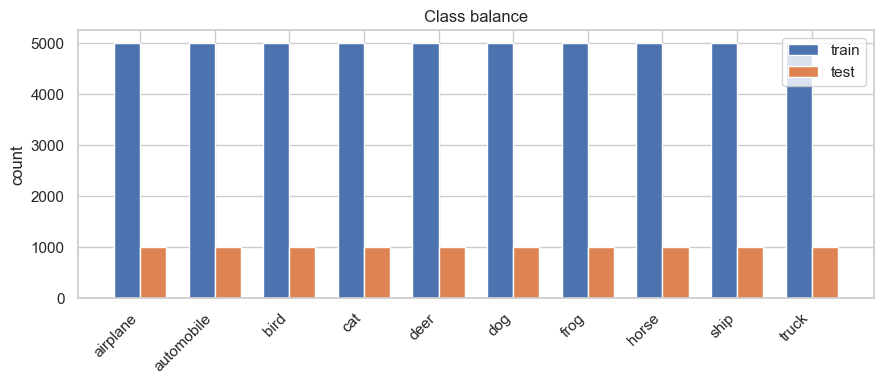
\includegraphics[width=0.7\linewidth]{images/cifar10_eda_class_balance.png}
\caption{Cân bằng lớp của CIFAR-10, tập train và test. Mỗi lớp có đúng
5.000 ảnh train và 1.000 ảnh test.}
\end{figure}

\begin{figure}[H]
\centering
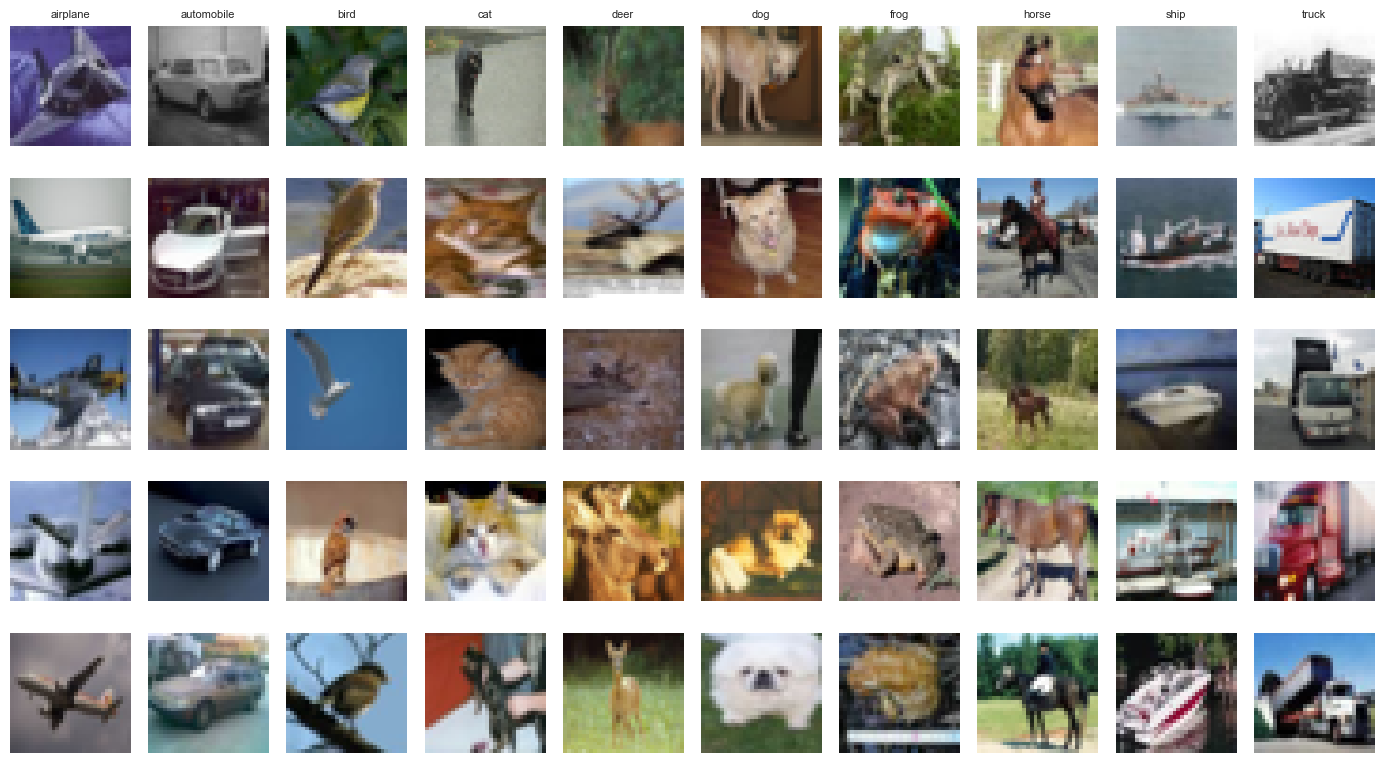
\includegraphics[width=\linewidth]{images/cifar10_eda_sample_grid.png}
\caption{Năm ảnh mẫu cho mỗi lớp. Đây là những bức ảnh màu thật chỉ ở độ
phân giải $32\times32$, đủ nhỏ để một số cặp lớp (ô tô/xe tải, mèo/chó)
thực sự mập mờ ngay cả với mắt người.}
\end{figure}

\begin{figure}[H]
\centering
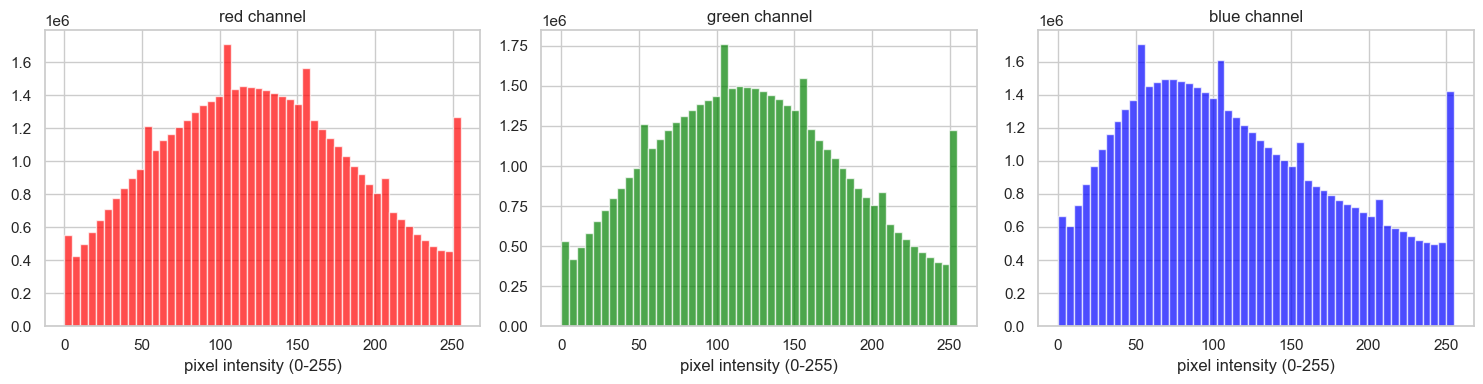
\includegraphics[width=\linewidth]{images/cifar10_eda_channel_hist.png}
\caption{Phân bố cường độ pixel theo từng kênh (đỏ, lục, lam) trước khi
chuẩn hóa. Cả ba kênh đều trải khắp toàn bộ khoảng 0-255 với hình dạng khá
tương đồng, khác với histogram một kênh của Fashion-MNIST, vốn có một đỉnh
áp đảo tại 0 do nền đen trơn.}
\end{figure}

\subsection{Biểu diễn dữ liệu}

Giá trị pixel được ép kiểu \code{float32} và chia cho 255. CIFAR-10 vốn
đã ở dạng channel-last, $(N, 32, 32, 3)$, khớp trực tiếp với layout mặc
định của Keras, không cần transpose; scratch và PyTorch thay vào đó dùng
một bản sao đã transpose sang channel-first, $(N, 3, 32, 32)$. Không cần
làm sạch thêm, cùng lý do benchmark đã tuyển chọn như Fashion-MNIST.

\subsection{Kiến trúc chung}

Cả ba cách cài đặt xây dựng cùng một mạng, là một thể hiện trực tiếp của
kiến trúc CNN mà tài liệu hướng dẫn của khóa học đã trình bày đầy đủ cho
đầu vào $3\times32\times32$:
\[
\resizebox{\linewidth}{!}{$3\times32\times32 \to \text{Conv}(3{\to}32, k{=}3, \text{pad}{=}1) \to \text{ReLU}
\to \text{MaxPool}(2) \to \text{Conv}(32{\to}64, k{=}3, \text{pad}{=}1) \to
\text{ReLU} \to \text{MaxPool}(2)$}
\]
\[
\to \text{Flatten} (64{\times}8{\times}8 = 4096) \to \text{Linear}(4096{\to}128)
\to \text{ReLU} \to \text{Linear}(128{\to}10)
\]
với dấu vết hình dạng, cho một batch kích thước $B$:
\[
\resizebox{\linewidth}{!}{$(B,3,32,32) \to (B,32,32,32) \to (B,32,16,16) \to (B,64,16,16) \to (B,64,8,8)
\to (B,4096) \to (B,128) \to (B,10)$}
\]
khớp chính xác với tiến trình hình dạng đã được trình bày trong tài liệu
hướng dẫn. Kích thước batch 256, 12 epoch, tốc độ học 0.05, và SGD thuần
túy được cố định một lần ở đây và tái sử dụng không đổi ở cả ba cách cài
đặt.

\subsection{Ba cách cài đặt}

\subsubsection{Viết tay, chỉ dùng NumPy}

Cách cài đặt scratch tái sử dụng đúng bộ máy
\code{conv2d\_forward}/\code{backward} (\code{im2col}),
\code{max\_pool2d\_forward}/\code{backward}, \code{relu()}, và
softmax-cross-entropy đã xây dựng cho Fashion-MNIST, được điều chỉnh tường
minh để nhận biết 3 kênh: shape của kernel đầu tiên là $(32, 3, 3, 3)$
thay vì $(32, 1, 3, 3)$, vì đầu vào giờ có ba kênh thay vì một. Một phép
kiểm tra gradient bằng số trên một mẫu tổng hợp có 3 kênh đầu vào xác nhận
lượt backward của convolution là đúng riêng cho trường hợp đa kênh, chứ
không chỉ trường hợp một kênh mà Fashion-MNIST đã kiểm chứng, trước khi
chạy huấn luyện đầy đủ. Bug chia dư $1/N$ ở lớp dense, đã được sửa cho
Fashion-MNIST, cũng đã được sửa ở đây từ trước khi notebook này được thực
thi lần nào, nên không có lần chạy huấn luyện nào ở đây bị ảnh hưởng bởi
nó. Gradient descent theo mini-batch (kích thước batch 256, 196 batch mỗi
epoch) huấn luyện trong 12 epoch.

\subsubsection{TensorFlow/Keras}

Cùng kiến trúc trở thành đúng hình dạng \code{Sequential} tám lớp như
Fashion-MNIST, với \code{Conv2D(32,3,...)} nhận trực tiếp đầu vào
$(32,32,3)$, không cần chuyển đổi thứ tự kênh vì CIFAR-10 vốn đã ở layout
Keras ưa thích. Được compile với \code{SGD(learning\_rate=0.05)} và
\code{SparseCategoricalCrossentropy(from\_logits=True)}, huấn luyện bằng
một lệnh gọi \code{model.fit(X\_train\_hwc, y\_train, batch\_size=256,
epochs=12)}. \code{model.summary()} báo cáo 545.098 tham số, khớp chính
xác với scratch.

\subsubsection{PyTorch}

Cùng kiến trúc trở thành một \code{nn.Module} (\code{Cifar10CNN}), có cấu
trúc giống hệt \code{FashionCNN} của Fashion-MNIST ngoại trừ số kênh đầu
vào của convolution đầu tiên (3 thay vì 1) và kích thước đặc trưng sau
flatten ($64 \times 8 \times 8 = 4096$ thay vì $64 \times 7 \times 7 =
3136$, vì đầu vào $32\times32$ lớn hơn của CIFAR-10 vẫn còn kích thước
không gian lớn hơn sau hai lần pooling stride-2 so với $28\times28$ của
Fashion-MNIST). Vòng lặp huấn luyện tường minh và \code{nn.CrossEntropyLoss()}
được giữ nguyên từ Fashion-MNIST. Số tham số kết quả, 545.098, khớp chính
xác với cả hai cách cài đặt còn lại.

\subsection{Bảng đối chiếu thành phần theo từng cách cài đặt}

\begin{table}[H]
\centering
\caption{CIFAR-10: bảng đối chiếu thành phần theo từng cách cài đặt}
\footnotesize
\begin{tabular}{@{}p{2.5cm}p{4.1cm}p{4.1cm}p{4.1cm}@{}}
\toprule
Thành phần & Scratch & Keras & PyTorch \\
\midrule
Tải dữ liệu & bộ tải của Keras, mảng NumPy dùng chung & giống nhau & giống nhau \\
Tiền xử lý & /255, reshape channel-first viết tay & /255, channel-last (giữ nguyên, không transpose) & /255, channel-first (đã transpose) \\
Định nghĩa mô hình & các hàm tường minh $+$ một dict tham số & \code{Sequential([...])} & lớp con \code{nn.Module} \\
Convolution & \code{conv2d\_forward}/\code{backward} (\code{im2col}, nhận biết 3 kênh) & \code{Conv2D(...)} & \code{nn.Conv2d(...)} \\
Activation & \code{relu()} & \code{activation="relu"} & \code{nn.ReLU()} \\
Pooling & \code{max\_pool2d\_forward}/\code{backward} & \code{MaxPooling2D(2)} & \code{nn.MaxPool2d(2)} \\
Flatten & \code{flatten\_forward}/\code{backward} (reshape) & \code{Flatten()} & \code{nn.Flatten()} \\
Lớp Dense/Linear & \code{linear\_forward}/\code{backward} & \code{Dense(...)} & \code{nn.Linear(...)} \\
Loss & softmax cross-entropy viết tay & \code{SparseCategorical}\allowbreak\code{Crossentropy(}\allowbreak\code{from\_logits=True)} & \code{nn.CrossEntropyLoss()} \\
Gradient & backprop viết tay & autodiff (ngầm định trong \code{fit}) & \code{loss.backward()} (autograd) \\
Optimizer & \code{W -= lr * dW} viết tay & \code{optimizer="sgd"} & \code{torch.optim.SGD(...)} \\
Vòng lặp huấn luyện & \code{for epoch / for batch} tường minh & \code{model.fit(...)} & \code{for epoch / for batch} tường minh \\
Đánh giá & các hàm đo chỉ số viết tay & tương đương \code{model.evaluate} (viết tay) & viết tay (\code{model.eval()}, no-grad) \\
Dự đoán & \code{forward(X\_test, params)} & \code{model.predict(...)} & \code{model(x\_test)} trong \code{torch.no\_grad()} \\
\bottomrule
\end{tabular}
\end{table}

\subsection{Đường cong huấn luyện và đánh giá}

\begin{figure}[H]
\centering
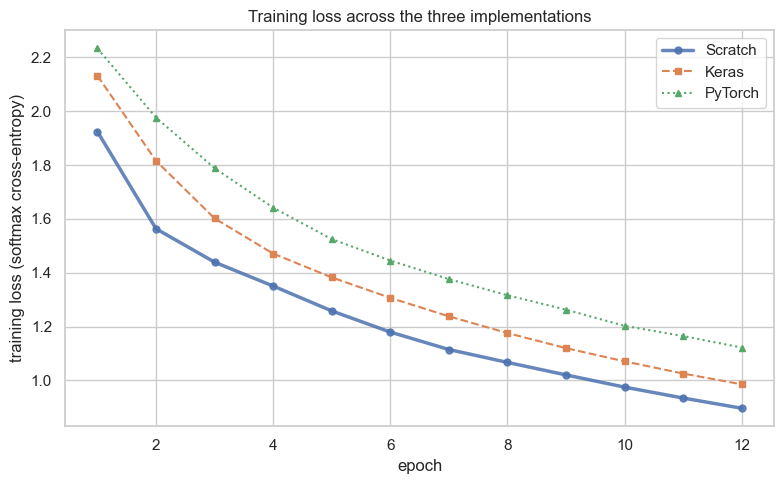
\includegraphics[width=\linewidth]{images/cifar10_compare_loss.png}
\caption{Loss huấn luyện của ba cách cài đặt.}
\end{figure}

\begin{figure}[H]
\centering
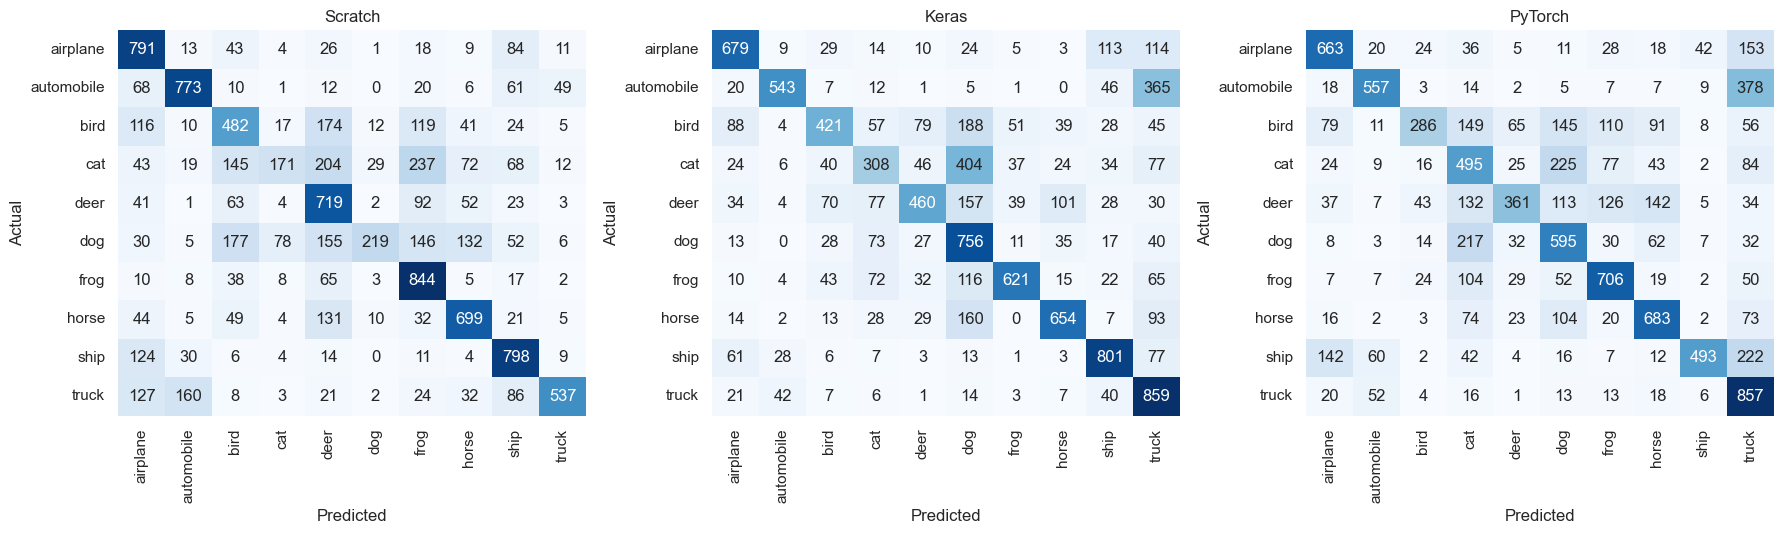
\includegraphics[width=\linewidth]{images/cifar10_compare_confmat.png}
\caption{Ma trận nhầm lẫn của ba cách cài đặt trên tập test CIFAR-10
(10.000 ảnh). Mèo/chó và ô tô/xe tải là các cặp bị nhầm lẫn nhiều nhất ở
cả ba, khớp với sự mập mờ về hình ảnh đã nêu ở lưới ảnh mẫu phía trên.}
\end{figure}

\begin{table}[H]
\centering
\caption{CIFAR-10: so sánh định lượng, tập test}
\label{tab:cifar-quant}
\begin{tabular}{lrrrrrr}
\toprule
Cách cài đặt & Tham số & T.gian train (s) & Loss cuối & Accuracy & Precision (macro) & Recall (macro) \\
\midrule
Scratch & 545.098 & 1.875,8 & 0.8965 & 0.6033 & 0.6335 & 0.6033 \\
Keras & 545.098 & 103,3 & 0.9854 & 0.6102 & 0.6477 & 0.6102 \\
PyTorch & 545.098 & 244,1 & 1.1220 & 0.5696 & 0.6163 & 0.5696 \\
\bottomrule
\end{tabular}
\end{table}

F1-macro cho cùng ba cách cài đặt, theo đúng thứ tự: 0.5794 (scratch),
0.6078 (Keras), 0.5655 (PyTorch).

\begin{figure}[H]
\centering
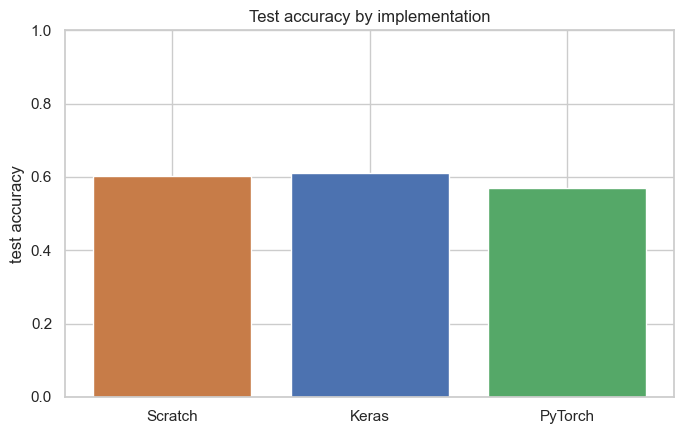
\includegraphics[width=0.6\linewidth]{images/cifar10_compare_accuracy.png}
\caption{Độ chính xác trên tập test theo từng cách cài đặt. Accuracy tuyệt
đối thấp hơn nhiều so với Fashion-MNIST — hệ quả dự kiến của một bài toán
thực sự khó hơn.}
\end{figure}

\begin{figure}[H]
\centering
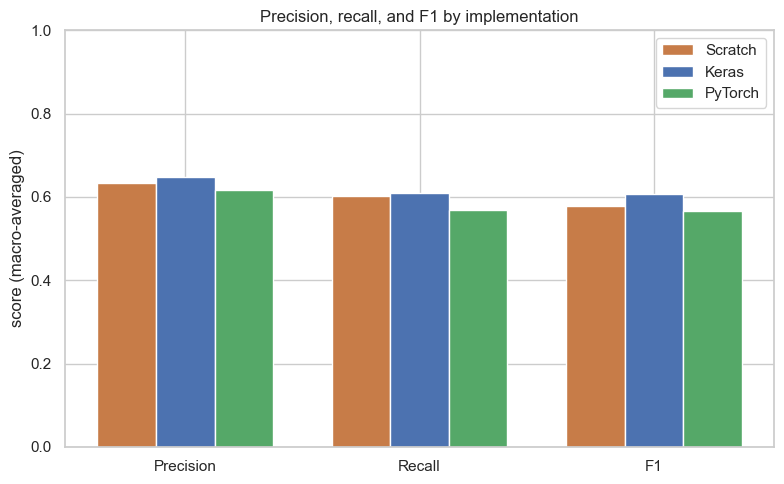
\includegraphics[width=0.7\linewidth]{images/cifar10_compare_prf1.png}
\caption{Precision, recall, và F1 (trung bình macro) theo từng cách cài
đặt.}
\end{figure}

\begin{figure}[H]
\centering
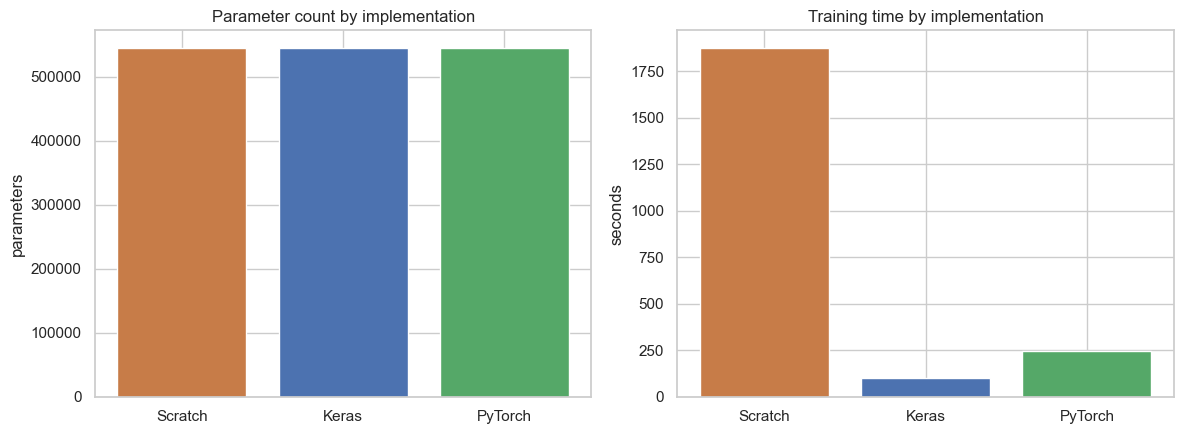
\includegraphics[width=\linewidth]{images/cifar10_compare_params_time.png}
\caption{Số lượng tham số (giống hệt nhau ở cả ba) và thời gian huấn luyện
theo từng cách cài đặt. Khoảng cách thời gian huấn luyện giữa scratch và
hai framework là rộng nhất trong ba ứng dụng của báo cáo này.}
\end{figure}

\subsection{Thảo luận so sánh}
\label{sec:cifar-compare}

Keras về đích nhỉnh hơn một chút ở cả accuracy (0.610) và F1 (0.608), với
scratch bám sát phía sau (0.603 accuracy, 0.579 F1) và PyTorch tụt lại
thêm một chút (0.570 accuracy, 0.566 F1). Cả ba nằm trong khoảng chênh
lệch khoảng bốn điểm phần trăm với nhau — cùng mức độ chênh lệch đã thấy
ở cả hai ứng dụng còn lại trong báo cáo này, phù hợp với việc đây là ba
cách cài đặt của cùng một kiến trúc chứ không phải ba mô hình khác nhau.
Accuracy tuyệt đối ở đây, quanh mức 60\%, thấp hơn nhiều so với mức gần
90\% của Fashion-MNIST với cùng kiến trúc, và điều đó là dự kiến: đây là
những bức ảnh màu thật được nén xuống $32\times32$ pixel, các cặp lớp như
mèo/chó và ô tô/xe tải thực sự khó phân biệt ngay cả ở độ phân giải đó, và
một mạng chỉ có hai lớp convolution, không data augmentation, và chỉ 12
epoch SGD thuần túy là một mô hình khiêm tốn cho một bài toán ở mức độ khó
này. Accuracy ở mức 60\% ở đây không phải dấu hiệu có gì bị lỗi; đây gần
như đúng là năng lực của kiến trúc này trên dữ liệu này khi không có các
kỹ thuật huấn luyện nâng cao — augmentation, nhiều epoch hơn, mạng lớn
hơn, optimizer tinh vi hơn — vốn bị cố tình bỏ qua để giữ cho ba cách cài
đặt dễ so sánh với nhau.

Thời gian huấn luyện lặp lại pattern đã thấy đầu tiên ở Fashion-MNIST:
scratch chậm hơn hẳn hai cách còn lại, và khoảng cách còn rộng hơn ở đây.
Scratch mất 1.875,8 giây (khoảng 31 phút) để huấn luyện. Keras mất 103,3
giây. PyTorch mất 244,1 giây. Scratch chậm hơn Keras khoảng 18,2 lần và
chậm hơn PyTorch khoảng 7,7 lần — một tỉ lệ rộng hơn so với 17,6x/6,9x của
Fashion-MNIST, dù mạng này chỉ có nhiều hơn một chút tham số (545.098 so
với 421.642). Điều đó cho thấy kích thước đầu vào và số kênh — ba kênh màu
thay vì một, và một ảnh $32\times32$ thay vì $28\times28$ — chứ không phải
số lượng tham số, mới là yếu tố thực sự chi phối chi phí convolution
\code{im2col} của scratch: cả hai thay đổi đều làm tăng khối lượng công
việc mà phép nhân ma trận của lớp convolution đầu tiên phải làm, và scratch
phải trả chi phí đó trực tiếp bằng thời gian thực tế mà không có tối ưu
hóa cấp framework nào để hấp thụ nó, trong khi các phép toán convolution
đã biên dịch của Keras và PyTorch scale mượt mà hơn nhiều. Đọc cùng với
Mục \ref{sec:fm-compare}, một tiến trình ba điểm rõ ràng xuất hiện xuyên
suốt ba ứng dụng của báo cáo này: ở MLP Diabetes (Mục
\ref{sec:diabetes-compare}), scratch có tốc độ tương đương các framework,
PyTorch thực ra chậm nhất; ở CNN ảnh xám, scratch chậm hơn Keras khoảng
17,6 lần; ở CNN ảnh RGB, scratch chậm hơn Keras khoảng 18,2 lần. Chi phí
thời gian huấn luyện của việc tự xây dựng mạng bằng tay tăng cụ thể theo
khối lượng công việc convolution thực sự mà kiến trúc yêu cầu, chứ không
phải chỉ theo số lượng tham số.

Framework nào ẩn nhiều nhất, và framework nào cho quyền kiểm soát nhiều
nhất, có cùng câu trả lời như Fashion-MNIST, với cùng lý do: Keras ẩn
convolution, pooling, lượt backward, và vòng lặp huấn luyện phía sau một
định nghĩa \code{Sequential} và một lệnh gọi \code{fit()}; PyTorch chỉ ẩn
lượt backward; scratch không ẩn gì cả. Pattern xuyên suốt ba ứng dụng của
báo cáo này giờ đã rõ ràng: chênh lệch accuracy giữa scratch, Keras, và
PyTorch luôn nhỏ, trong khoảng vài điểm phần trăm, bất cứ khi nào kiến
trúc thực sự được giữ cố định — đây là kết quả dự kiến và là mục đích
chính của việc xây dựng cùng một mạng ba lần. Ngược lại, chênh lệch thời
gian huấn luyện có thể rất lớn và phụ thuộc mạnh vào việc kiến trúc thực
sự yêu cầu phần cứng làm gì — không đáng kể với một mạng fully-connected
nhỏ, lớn và gắn liền cụ thể với khối lượng công việc convolution đối với
một CNN. Một cách cài đặt NumPy viết tay từ đầu, dù đúng đến đâu, cũng
không thể sánh được với tối ưu hóa cấp toán tử của một framework trưởng
thành cho một phép toán như convolution, trừ khi tự áp dụng cùng loại công
việc tối ưu hóa cấp thấp mà các framework đó đại diện.

\newpage
% ---------------------------------------------------------------------
\section{So sánh xuyên suốt các ứng dụng}
\label{sec:cross}
% ---------------------------------------------------------------------

Bảng \ref{tab:cross-app} tóm tắt cả ba ứng dụng theo độ chính xác trên tập
test — chỉ số chính được dùng xuyên suốt báo cáo này vì không ứng dụng nào
trong ba ứng dụng là bài toán hồi quy — ở cả ba cách cài đặt. Mỗi ô trong
bảng là một phép chuyển vị của các bảng kết quả theo từng ứng dụng ở các
Mục \ref{sec:diabetes}, \ref{sec:fashion}, và \ref{sec:cifar10}, không
phải phân tích mới.

\begin{table}[H]
\centering
\caption{Tóm tắt xuyên suốt ứng dụng: độ chính xác trên tập test, 3 ứng
dụng x 3 cách cài đặt}
\label{tab:cross-app}
\begin{tabular}{llrr}
\toprule
Ứng dụng & Cách cài đặt & Tham số & Accuracy \\
\midrule
\multirow{3}{*}{Diabetes}
  & Scratch & 2.177 & 0.7310 \\
  & Keras & 2.177 & 0.7533 \\
  & PyTorch & 2.177 & \textbf{0.7819} \\
\midrule
\multirow{3}{*}{Fashion-MNIST}
  & Scratch & 421.642 & \textbf{0.8973} \\
  & Keras & 421.642 & 0.8603 \\
  & PyTorch & 421.642 & 0.8660 \\
\midrule
\multirow{3}{*}{CIFAR-10}
  & Scratch & 545.098 & 0.6033 \\
  & Keras & 545.098 & \textbf{0.6102} \\
  & PyTorch & 545.098 & 0.5696 \\
\bottomrule
\end{tabular}
\end{table}

\noindent\textit{Chữ đậm đánh dấu cách cài đặt thắng ở mỗi ứng dụng. Số
lượng tham số giống hệt nhau ở cả ba cách cài đặt trong cùng một ứng dụng,
được xác nhận bằng một phép \code{assert} trực tiếp trong mọi notebook.}

\begin{table}[H]
\centering
\caption{Thời gian huấn luyện xuyên suốt ứng dụng, giây, 3 ứng dụng x 3
cách cài đặt}
\label{tab:cross-time}
\begin{tabular}{lrrr}
\toprule
Ứng dụng & Scratch & Keras & PyTorch \\
\midrule
Diabetes & 69,4 & \textbf{24,7} & 311,0 \\
Fashion-MNIST & 1.330,5 & \textbf{75,6} & 191,5 \\
CIFAR-10 & 1.875,8 & \textbf{103,3} & 244,1 \\
\bottomrule
\end{tabular}
\end{table}

\noindent\textit{Chữ đậm đánh dấu cách cài đặt nhanh nhất ở mỗi ứng dụng.
Keras nhanh nhất ở mọi ứng dụng. Scratch chỉ nhanh hơn trong hai cách cài
đặt còn lại (không tính Keras) duy nhất ở Diabetes — mạng MLP nhỏ của nó;
scratch là cách cài đặt chậm nhất với khoảng cách lớn ở cả hai ứng dụng
CNN.}

Không có cách cài đặt nào thắng ở mọi ứng dụng, và cách cài đặt thắng với
khoảng cách rộng nhất — PyTorch ở Diabetes — cũng chính là cách cài đặt
chậm nhất ở đúng ứng dụng đó, một minh chứng trực tiếp rằng accuracy và
tốc độ huấn luyện là hai trục độc lập ở đây, chứ không phải hai góc nhìn
của cùng một chất lượng nền tảng.

% ---------------------------------------------------------------------
\section{Thảo luận}
\label{sec:discussion}
% ---------------------------------------------------------------------

\subsection{Luận điểm "cùng kiến trúc, khác mức độ trừu tượng" có thực sự
đúng không?}

Có, trên trục mà nó tuyên bố mạnh mẽ nhất. Số lượng tham số của mọi ứng
dụng khớp chính xác ở cả ba cách cài đặt, được xác minh bằng một phép
\code{assert} trực tiếp trong mỗi notebook chứ không phải chỉ giả định, và
độ chênh lệch accuracy của mọi ứng dụng giữa ba cách cài đặt luôn nằm
trong khoảng bốn đến năm điểm phần trăm — loại khoảng cách có thể giải
thích được bằng sự khác biệt khởi tạo và nhiễu thông thường của việc huấn
luyện một kiến trúc cố định, chứ không phải bằng chứng cho thấy một cách
cài đặt nào đó vốn dĩ học tốt hơn. Thứ hạng thay đổi liên tục ở Bảng
\ref{tab:cross-app} — PyTorch ở Diabetes, scratch ở Fashion-MNIST, Keras ở
CIFAR-10 — chính là pattern mà luận điểm này dự đoán: nếu cách cài đặt
"cùng kiến trúc" của một framework cụ thể nào đó bí mật là một mô hình
mạnh hơn, nó sẽ thắng liên tục, chứ không phải thay phiên nhau thắng.

\subsection{Nơi các mức độ trừu tượng thực sự phân kỳ}

Thời gian huấn luyện là nơi ba mức độ trừu tượng thôi không còn hành xử
như những góc nhìn có thể hoán đổi cho nhau của cùng một phép tính. Ở MLP
Diabetes, một mạng dense nhỏ và đầy đủ, scratch và Keras huấn luyện trong
khoảng thời gian tương đương, và PyTorch thực ra là cách cài đặt chậm
nhất, với chi phí cố định của việc xây dựng đồ thị autograd theo từng
batch quá lớn để một mạng 2.177 tham số có thể khấu hao hết bằng khối
lượng tính toán thực sự của nó. Một khi convolution thực sự xuất hiện,
Fashion-MNIST và CIFAR-10, pattern đó đảo ngược hoàn toàn: scratch trở
thành cách cài đặt chậm nhất với một khoảng cách rộng và ngày càng rộng
hơn (17,6x Keras ở Fashion-MNIST, 18,2x Keras ở CIFAR-10), bởi vì một
convolution \code{im2col} viết tay từ đầu, dù được cài đặt đúng đắn đến
đâu và dù nhanh hơn vòng lặp theo vị trí naive mà nó thay thế đến đâu, vẫn
chỉ là NumPy thuần túy được phát ra từ một vòng lặp huấn luyện Python,
không có tối ưu hóa cấp toán tử nào của một framework trưởng thành dành
riêng cho convolution. Khoảng cách này lại càng rộng thêm giữa hai ứng
dụng CNN, tỉ lệ theo kích thước đầu vào và số kênh (CIFAR-10's
$32\times32\times3$ so với $28\times28\times1$ của Fashion-MNIST), chứ
không theo số lượng tham số, vốn chỉ tăng khiêm tốn giữa hai ứng dụng
(545.098 so với 421.642). Khả năng hiển thị, tính đúng đắn, và tốc độ là
ba thuộc tính riêng biệt của một cách cài đặt, và các con số đo được của
chính dự án này cho thấy chúng đánh đổi lẫn nhau đúng theo hướng mà
Lecture 04 dự đoán — càng nhiều hai thuộc tính đầu thì càng tốn nhiều thời
gian thực tế hơn.

\subsection{Điều mà việc tự viết từng vòng lặp huấn luyện bằng tay đã phơi
bày}

Hai phát hiện đã lộ ra cụ thể vì bài tập này giữ cho cách cài đặt scratch
hoàn toàn minh bạch thay vì tin tưởng vào một lệnh gọi \code{fit()} đóng
gói, và cả hai đều đáng được nêu tên vì một framework sẽ âm thầm hấp thụ
chúng. Thứ nhất, giá trị loss của PyTorch ở ứng dụng Diabetes (Mục
\ref{sec:diabetes-compare}) nằm trên một thang giá trị số thực sự khác
biệt so với scratch và Keras — không phải vì PyTorch huấn luyện một mô
hình tệ hơn, mà vì \code{BCEWithLogitsLoss(pos\_weight=...)} chỉ tái cân
bằng trọng số cho số hạng loss của lớp dương, trong khi trọng số tự tính
tay của scratch và \code{class\_weight} của Keras đều tái cân bằng trọng
số cho mọi dòng. Ba framework cùng cung cấp thứ trông như cùng một tính
năng được đặt tên — cân bằng trọng số lớp — nhưng thực tế tham số hóa nó
khác nhau bên dưới, đúng như cảnh báo của chính Lecture 04 rằng tên gọi
khác nhau không ngụ ý khái niệm khác nhau, đọc theo chiều ngược lại: đôi
khi cùng một cái tên lại che giấu một khác biệt cơ chế thực sự, và cách
duy nhất để biết là kiểm tra code, chứ không phải tin vào cái tên. Thứ
hai, cell kiểm tra gradient của chính cách cài đặt scratch ở Fashion-MNIST
đã bắt được một bug thật trong quá trình phát triển — một phép chia dư
$1/N$ trong lượt backward của lớp dense âm thầm làm co nhỏ mọi gradient
của lớp dense, vô hình từ bên ngoài vì mạng vẫn huấn luyện được và vẫn cho
ra một đường cong loss trông hợp lý; chỉ việc so sánh gradient tính bằng
giải tích với một xấp xỉ sai phân hữu hạn bằng số, theo từng layer, mới
phơi bày nó ra. Cả hai phát hiện đều là phần thưởng trực tiếp của việc tự
xây dựng optimizer, loss, và phép tính gradient bằng tay thay vì import
chúng: một cách cài đặt đóng gói sẽ hấp thụ cả hai vấn đề này mà không bao
giờ để nó lộ ra như một điều cần giải thích.

% ---------------------------------------------------------------------
\section{Kết luận}
% ---------------------------------------------------------------------

Báo cáo này đã xây dựng ba hệ thống thông minh — sàng lọc nguy cơ tiểu
đường (MLP), nhận diện trang phục Fashion-MNIST (CNN), và nhận diện vật
thể CIFAR-10 (CNN) — và với mỗi hệ thống, cài đặt một kiến trúc duy nhất
ba lần riêng biệt: viết tay bằng NumPy, với mọi lượt forward, loss, lượt
backward, và cập nhật tham số được suy ra và viết bằng tay; bằng
TensorFlow/Keras; và bằng PyTorch. Ở cả ba cách cài đặt, số lượng tham số
của mỗi ứng dụng khớp chính xác và độ chênh lệch accuracy của mỗi ứng dụng
luôn nằm trong vài điểm phần trăm — cùng nhau xác nhận luận điểm trung tâm
của Lecture 04 rằng kiến trúc ở mức khái niệm giữ nguyên xuyên suốt các
mức độ trừu tượng và chỉ có cách biểu đạt nó là thay đổi. Ngược lại, thời
gian huấn luyện thực sự phân kỳ, và phân kỳ với khoảng cách lớn một khi có
convolution thực sự tham gia: một cách cài đặt NumPy viết tay từ đầu, dù
đúng đắn đến đâu, đơn giản là không thể sánh được với tối ưu hóa cấp toán
tử của một framework trưởng thành cho một phép toán như convolution — một
cái giá thực sự của việc hiển thị toàn bộ mà lượt forward của một MLP nhỏ
không bao giờ để lộ ra nhưng của một CNN thì có, và cái giá đó còn tăng
thêm theo kích thước đầu vào và số kênh chứ không phải theo số lượng tham
số. Việc giữ cho vòng lặp huấn luyện và phép tính loss của mỗi cách cài
đặt hoàn toàn minh bạch, thay vì dựa vào một lệnh gọi \code{fit()} đóng
gói, cũng chính là điều đã phơi bày hai phát hiện cụ thể mà một framework
lẽ ra đã hấp thụ mà không để lại dấu vết: cơ chế cân bằng trọng số lớp
\code{pos\_weight} của PyTorch scale loss huấn luyện khác với cách cân
bằng đối xứng của scratch và Keras dù cùng chia sẻ mục tiêu cân bằng
trọng số, và một bug chia dư trong lượt backward viết tay mà chỉ một phép
kiểm tra gradient bằng số, so sánh gradient suy ra bằng tay với một xấp xỉ
sai phân hữu hạn, mới có thể bắt được. Cả hai chi tiết này chỉ hiện ra
được với người đã tự viết từng gradient bằng tay — đúng là phần thưởng mà
việc xây dựng một CNN từ đầu được thiết kế để mang lại.

% ---------------------------------------------------------------------
\section{Khả năng tái lập}
% ---------------------------------------------------------------------

\subsection{Môi trường}

\begingroup\sloppy\emergencystretch=3em
Cả ba notebook đều được xây dựng và chạy trong một môi trường ảo riêng tại
\texttt{assignment\_04/.venv} (Python 3.10.11, đăng ký làm Jupyter kernel
\texttt{assignment\_04}), với các phiên bản package chính sau: numpy,
pandas, scikit-learn (chỉ dùng cho metric), matplotlib, seaborn, jupyter,
nbconvert, nbformat, nbclient, tensorflow 2.21.0, torch 2.14.0+cpu,
torchvision 0.29.0+cpu. Các gói PyTorch/torchvision bản CPU-only được cài
đặt một cách có chủ đích, để việc so sánh thời gian huấn luyện giữa ba
cách cài đặt không bị nhiễu bởi việc một cách cài đặt nào đó chạy trên một
lớp thiết bị (device class) khác với các cách còn lại.
\code{RANDOM\_SEED = 42} được cố định trong mọi notebook cho mọi lần chia
tập, xáo trộn, và khởi tạo trọng số (\code{np.random.seed}, hàm
\code{random.seed} của Python, \code{tf.random.set\_seed}, và
\code{torch.manual\_seed}, tất cả được đặt cùng nhau).
\par\endgroup

\subsection{Chạy lại một notebook từ đầu đến cuối}

Notebook của mỗi ứng dụng đều độc lập (self-contained) và có thể được chạy
lại từ thư mục riêng của nó bằng:
\begin{footnotesize}
\begin{verbatim}
../.venv/Scripts/python.exe -m jupyter nbconvert \
    --to notebook --execute --inplace \
    notebook/<app>.ipynb --ExecutePreprocessor.timeout=1800
\end{verbatim}
\end{footnotesize}
thay \texttt{<app>} bằng \texttt{diabetes}, \texttt{fashion\_mnist}, hoặc
\texttt{cifar10}. Fashion-MNIST và CIFAR-10 tự động tải dữ liệu qua
\code{keras.datasets} ở lần chạy đầu tiên, không cần bước tải thủ công từ
Kaggle, khác với các file CSV của ứng dụng Diabetes, vốn phải đã có sẵn
trong \texttt{diabetes/data/}. Mỗi notebook kết thúc bằng việc lưu cả ba
artifact đã huấn luyện vào thư mục \texttt{model/} riêng của nó:
\begin{itemize}[nosep]
  \item \texttt{scratch\_weights.npz}: tham số đã huấn luyện của cách cài
    đặt scratch.
  \item \texttt{keras\_model.keras}: mô hình Keras đã huấn luyện.
  \item \texttt{pytorch\_model.pt}: state dict của mô hình PyTorch đã
    huấn luyện.
  \item \texttt{feature\_names.joblib} (chỉ Diabetes): thứ tự cột đặc
    trưng sau khi mã hóa.
  \item \texttt{input\_schema.json}: tài liệu mô tả các trường đầu vào và
    nhãn mục tiêu.
\end{itemize}
theo sau bởi một cell nạp-lại-và-xác-nhận (reload-and-verify), nạp lại cả
ba artifact và xác nhận dự đoán của chúng khớp với các phiên bản trong bộ
nhớ được tính trong cùng lần chạy đó. Bài tập này không bao gồm bất kỳ
tầng API, web, hay mobile nào, nên không cần thêm lệnh chạy nào ngoài việc
thực thi notebook.

\end{document}
